%%%%%%%%%%%%%%%%%%%%%%%%%%%%%%%%%%%%%%%%%%%%%%%%%%%

\documentclass[metals,article,accept,pdftex,moreauthors]{Definitions/mdpi}

%=================================================================
% MDPI internal commands - do not modify
\firstpage{1} 
\makeatletter 
\setcounter{page}{\@firstpage} 
\makeatother
\pubvolume{1}
\issuenum{1}
\articlenumber{0}
\pubyear{2023}
\copyrightyear{2023}
\externaleditor{Academic Editor: Firstname Lastname}
\datereceived{29 September 2023} 
\daterevised{20 October 2023} % Comment out if no revised date
\dateaccepted{ } 
\datepublished{ } 
%\datecorrected{} % For corrected papers: "Corrected: XXX" date in the original paper.
%\dateretracted{} % For corrected papers: "Retracted: XXX" date in the original paper.
\hreflink{https://doi.org/} % If needed use \linebreak
%\doinum{}
%\pdfoutput=1 % Uncommented for upload to arXiv.org

%=================================================================

%%\usepackage{subcaption}
%%\usepackage[labelformat=simple]{subcaption}
%%\renewcommand\thesubfigure{\alph{subfigure}}
%\DeclareCaptionLabelFormat{subcaptionlabel}{\normalfont(\textbf{#2}\normalfont)}
\usepackage{placeins}
\usepackage{acronym}
%\usepackage{subfigure}
%\makeatletter
%\renewcommand{\@thesubfigure}{\normalsize(\textbf{\alph{subfigure}})}
%\makeatother
\usepackage[labelformat=simple]{subcaption}
\renewcommand\thesubfigure{\alph{subfigure}}
\DeclareCaptionLabelFormat{subcaptionlabel}{\normalfont(\textbf{#2}\normalfont)}
\captionsetup[subfigure]{labelformat=subcaptionlabel}


%\usepackage[commentmarkup=footnote, authormarkup=none,
%	defaultcolor=red,
%	final
%	]{changesManual}

% \doublespacing


% [Searching for unknown material properties for AM simulations]
% \Title{\colorbox{green}{Application of} Mathematical Search Algorithms for Unknown Material Properties in Additive Manufacturing Simulations}
% Updated the title to be more concise
\Title{Searching for unknown material properties for AM simulations}

%MDPI Important Information:
%1. The initial layout for your manuscript was done by our layout team. Please do not change the layout, otherwise we cannot proceed to the next step.
%2. Please do not delete our comments.
%3. Please revise and answer all questions that we proposed, such as: “It should be italic”; “I confirm”; “I have checked and revised all.”
%4. Please directly correct on this version.
%5. Please make sure that all the symbols in the paper are of the same format.


% \TitleCitation{Application of Mathematical Search Algorithms for Unknown Material Properties in Additive Manufacturing Simulations}
\TitleCitation{Searching for unknown material properties for AM simulations}

\newcommand{\orcidauthorA}{0000-0002-5929-8345} 
\newcommand{\orcidauthorB}{0000-0002-4360-5013}
\newcommand{\orcidauthorC}{0000-0002-4848-2817} 
\newcommand{\orcidauthorD}{0000-0001-9505-0841} 

% Authors, for the paper (add full first names)
\Author{\hl{Aaron Flood} %MDPI: 1. Please carefully check the accuracy of names and affiliations; 2. Please add aff number of Aaron Flood
 *$^{1}$\orcidA{}, 
%  aff has been added
 Rachel Boillat $^{1}$\orcidB{}, 
 \hl{Sriram Praneeth Isanaka} %MDPI: The name of this author is different from the submitting system. Please confirm which one is correct.
%  Name has been fixed, thanks for the catch
 $^{1}$\orcidC{}
 and Frank Liou $^{1}$\orcidD{}}

\AuthorNames{Aaron Flood, Rachel Boillat, Sriram Praneeth Isanaka and Frank Liou}

\AuthorCitation{Flood, A.; Boillat, R.; Isanaka, S.; Liou, F.}

% \address{%
% $^{1}$ \quad \hl{Affiliation 1;}
% %MDPI: 1. please add affs 1-3; please note that affs 1-3 could not be same as Current address, if they are same, please remove Current address part 2. Please add affiliations of  All authors, provided information should be arranged from subordinate to superior. After affiliation, please add city, post code and country in all affiliations
%  rmb8t6@mst.edu\\
% $^{2}$ \quad \hl{Affiliation 2;} sihyd@mst.edu\\
% $^{3}$ \quad \hl{Affiliation 3;} liou@mst.edu}

\address{%
	$^{1}$ \quad Department of Mechanical and Aerospace Engineering, Missouri University of Science and Technology, Rolla, MO 65409, USA. rmb8t6@mst.edu (R.B); sihyd@mst.edu (S.P.I.); liou@mst.edu (F.L.)
}

\corres{Correspondence: ajfrk6@mst.edu}

% Current address and/or shared authorship
% \firstnote{These authors contributed equally to this work.}% MDPI: The number of co-authors with note “These authors contributed equally to this work” is recommended to no more than 2. But this paper, all authors has this note, please modify and confirm
% This has been removed due to misunderstanding on authors part.

% \secondnote{Current address: \hl{Department} %MDPI: The provided information should be arranged from subordinate to superior, please confirm we revised the order
%  of Mechanical and Aerospace Engineering, Missouri University of Science and Technology, 194 Toomey Hall, Rolla, MO 65409, USA.} 
% This has been removed due to misunderstanding how the author section was to go



\keyword{additive manufacturing (AM); mathematical modeling; mathematical search; material properties; aluminum; additive manufacturing (AM) simulation; input parameter optimization}
%\newcommand{\degree}{$^\circ$}
\graphicspath{{images/}}


% \usepackage{amsmath}
\acrodef{DED}{directed energy deposition}
\acrodef{AM}{additive manufacturing}
\acrodef{EDM}{electrical discharge machine}
\acrodef{BPP}{beam parameter product}
\acrodef{PBF}{powder bed fusion}
\acrodef{ML}{machine learning}
\acrodef{FFF}{fused filament fabrication}
\acrodef{FEA}{finite element analysis}




\abstract{Additive manufacturing (AM) simulations are effective for materials that are 
well characterized and published; however, for newer or proprietary materials, they 
cannot provide accurate results due to the lack of knowledge of the material properties. 
This work demonstrates the process of the application of mathematical search algorithms 
to develop an optimized material dataset which results in accurate simulations for the 
laser \ac{DED} process. This was performed by first using a well-characterized material, 
Ti-64, to show the error in the predicted melt pool was accurate, and the error was found to be less than two 
resolution steps.  % English Editor: Please verify that the intended meaning has been 
%retained.
% updated line 135 to keep the desired meaning
Then, for 7000-series aluminum using a generic material property dataset from sister 
alloys, the error was found to be over 600\%. The Nelder--Mead search algorithm was 
then applied to the problem and was able to develop an optimized dataset that had a 
combined width and depth error of just 9.1\%, demonstrating that it is possible to develop 
an optimized material property dataset that facilitates more accurate simulation of an 
under-characterized~material.}


\begin{document}

\section{Introduction}
\label{introAMsim}

Additive manufacturing (AM) is an emerging manufacturing technique that has the 
potential to revolutionize manufacturing.  To realize this revolution, it is necessary to be 
able to produce components reliably and to understand the process well enough to ensure 
that builds are consistent enough that the performance of the completed build can be 
guaranteed.  To execute this, researchers and manufacturers have turned to mathematical 
modeling to understand the process~\cite{neittaanmakiImpactScientificComputing2023}.
This body of work focuses solely on increasing the accuracy of thermal modeling of the 
process; however, the thermal cycling that a build experiences affects the resulting 
microstructure~\cite{qianSubrapidSolidificationStudy2020, 
weiMechanisticModelsAdditive2020, ansariSelectiveLaserMelting2022}, residual stress and 
distortion~\cite{weiMechanisticModelsAdditive2020, ningAnalyticalModelingPart2020, 
promoppatumPartScaleEstimation2021}, and porosity of the 
build~\cite{ningAnalyticalModelingPart2020a, wangPredictionLackoffusionPorosity2021, 
linProcessOptimizationDirected2020}.  If the accuracy of the underlying thermal modeling 
prediction can be improved, then the subsequent properties can be more accurately 
modeled as well.

The differences in simulation techniques can vary based on the desired response from the simulation and the underlying assumptions that were made during the development of the models.
One example of this can be seen when comparing the mathematical models developed by 
Wang and Chen~\cite{wangClosedLoopHighFidelitySimulation2021}, Roy and 
Wodo~\cite{royDatadrivenModelingThermal2020}, and Moges 
et~al.~\cite{mogesHYBRIDMODELINGAPPROACH2020}.  They all attempted to model 
roughly the same aspect of the build but took very different approaches.
Wang and Chen~\cite{wangClosedLoopHighFidelitySimulation2021} took a purely 
physics-based approach to the solution and developed a model from a fundamental 
physics-first principle approach for the physical process being modeled. This was 
performed for Ti-64 and was able to obtain an accuracy of between 3.6\% and 9.0\%.
On the contrary, Roy and Wodo~\cite{royDatadrivenModelingThermal2020} used a 
data-driven model that used a breadth of data to develop a mathematical model that 
properly predicted the material behavior. This model was applied to the plastic \ac{FFF} 
process due to the volume of data required.  It would be possible to develop the model for 
a metal process, though it could become cost-prohibitive quickly.
In between these models exists Moges 
et~al.~\cite{mogesHYBRIDMODELINGAPPROACH2020}, which attempted to marry the 
two approaches and develop a physics-based model that uses data to improve the 
accuracy. This was able to produce results with an average relative error of 7.58\% for 
Inconel 625.


The one unifying characteristic of these, and all mathematical models, is the need for the 
inclusion of a dataset that defines the behavior of the material being investigated; this is 
colloquially referred to as the material properties.  These material properties can vary in 
the literature and this variance in values can lead to a discrepancy in simulation 
results~\cite{daryabeigiThermalPropertiesAccurate2011}.
This need for input material properties extends to surrogate models that have been developed, such as \ac{ML} models, which will also require the inclusion of these material properties to properly predict the outcome~\cite{zhuMachineLearningMetal2020, zobeiryPhysicsinformedMachineLearning2021, mengMachineLearningAdditive2020, wangMachineLearningAdditive2020}.

Though variation exists in the literature, values can be found and used when the material 
is well characterized and published.  An example of a well-published material is Ti-64, 
where it is easy to find literature that reports the material properties such as Welsch 
et~al.~\cite{welschgerhard_1993}, Boivineau et~al.~\cite{boivineau_2006}, and Fan and 
Liou~\cite{fan_2012}.  However, for materials that are not well characterized or published, 
such as specific aluminum alloys, it can be very challenging to find some properties, as 
reported by Lindberg~\cite{lundberg_material_1994} and Leitner 
et~al.~\cite{leitner_thermophysical_2017}.  There arises a need to determine a complete 
dataset of the material properties, or at a minimum, develop a dataset that produces the 
most accurate simulation results. 
This can be accomplished by expending the necessary resources to measure the needed properties using advanced equipment.
This process can be expensive and time-consuming, which has led to the development of 
material simulations that attempt to predict the material properties, such as 
JMatPro~\cite{jmatpro}.  Though faster and cheaper than experimental results, they, like 
all simulations, have an error that is associated with them; this has been reported by Liu 
et~al.~\cite{liuStudyPredictionTensile2020}, Chen 
et~al.~\cite{chenMicrostructurePropertiesIronbased2023}, and Geng 
et~al.~\cite{gengDatadrivenMachineLearning2022}.  Using these values alone can lead to 
unknown errors stacking up in the \ac{AM} models.
This problem also applies to materials where the tolerances for alloying elements is so 
wide that specimens of the same alloy can have different material properties.  

To develop a dataset that produces accurate \ac{AM} simulation results, an optimization routine can be used as a search algorithm to determine the dataset that produces the most realistic results.  This can be used to develop a dataset for a new alloy or for a specific batch of stock that has been procured from a supplier. 


This work will aim to address one of the current desires in metal \ac{AM} which is to be 
able to produce parts out of aluminum.  The desire is evident by the volume of effort being 
applied to aluminum \ac{AM}~\cite{qiHighStrengthLi2020, 
weissImprovedHighTemperatureAluminum2019, 
weissDevelopmentsAluminumScandiumCeramicAluminumScandiumCerium2019}.  The 
challenge associated with this stems from the wide range of alloys that have wildly 
varying material properties and are not well published.  One of the weldable high-strength 
alloys that have been targeted for metal \ac{AM} is 
7050~\cite{singhAdditiveManufacturing4047}.  Though the material is widely available, 
the temperature-dependent material properties are not readily available.  
This work will perform an optimization routine on the material dataset for the 7050 
aluminum alloy to enable more accurate simulation results.  This will be performed by 
validating the model on the well-characterized Ti-64 material, showing the model's 
effectiveness.  Then, utilizing sister alloys, a generic material property dataset will be 
found in the literature.  The search algorithm will then be applied to generate an optimal 
input property dataset.  These optimized material properties will then be used with a 
range of 
laser parameters and compared experimentally to show their effectiveness over a 
processing window.




\section{Materials and Methods}
\label{methodsOverview}

This body of work begins by describing the thermal model which was developed to 
simulate the metal \ac{AM} deposition process for any metal where the material 
properties could be determined.  This model is then validated using a well-characterized 
material, Ti-64.  Upon validation of the thermal model, it is applied to a generic aluminum 
alloy, and then experimentation is used to determine if the results are a good 
representation of the physical process.  When found to be inaccurate, a mathematical 
search algorithm was applied to the input parameters to increase the accuracy of the 
model's results.  Lastly, the optimal input dataset was validated by comparing the 
simulated results to experimental results with a range of laser scan speeds and power 
levels for the targeted aluminum alloy.

\subsection{Simulation Description}
\label{model_description}

The model used in this study was developed at the Missouri University of Science and 
Technology.
This simulation has the express goal of being efficient while still holding to physics 
models.  To accomplish this, it heavily leverages GPU processing by utilizing image 
processing techniques.  The simulation was developed with the laser \ac{DED} processes 
in mind; however, it was developed in a modular manner such that it can be applied to 
most \ac{AM} processes. 

The model is a voxel-based simulation, which forgoes the calculation of the fluid flow and focuses on heat transfer and material insertion.  This decision was based on past simulation development experience, where it was determined that the calculation of the fluid flow was the most computationally expensive part of the simulation.   

The governing equations of the model developed can be seen in Equations 
\eqref{eqn:conduction}--\eqref{eqn:laser_absorption}, which describe the flow of heat 
from conduction, convection, and radiation, and laser absorption, 
respectively~\cite{Han2012}.
\begin{equation}
\label{eqn:conduction}
\centering
\rho c_p \frac{\partial T}{\partial t}=k \left(\frac{\partial^2 T}{\partial x^2} +\frac{\partial^2 T}{\partial y^2}+\frac{\partial^2 T}{\partial z^2} \right)
\end{equation}
	\begin{equation}
	\label{eqn:conv-rad}
	\centering
	k \frac{\partial T}{\partial n}=-h (T_s-T_a) - \varepsilon \sigma ({T_s}^4-{T_a}^4) + \phi(x, y, z) + \rho c \frac{\partial T}{\partial t}
	\end{equation}
		\begin{equation}
		\label{eqn:laser_absorption}
		\centering
		\phi(x,y,z) = H(z) \alpha \phi_0 \sqrt{1-\frac{x^2}{r_0^2} -\frac{y^2}{r_0^2}}
		\end{equation}
\hl{In these} %MDPI: Please confirm whether the format without indentation is necessary; highlight below same as this
% This is meant to be a continuation of the previous paragraph which does not appear to be properly adjusting.  The authors defer to the editors as to the proper typsetting for this
equations, $\rho$ is density, $c_p$ is specific heat, $k$ is thermal conductivity, $h$ is 
 convection coefficient, $\varepsilon$ is emissivity, $\sigma$ is the Stefan--Boltzmann 
 constant, and n is the unit (outward) normal vector of a point at location \hl{$(x, y, 
 z)$}%MDPI: please confirm if format of letters should be unified with equations, whether need italic, please modify
 that is located on the outer surface of the component, $r_0$ is the radius of the laser beam, $\alpha$ is the absorption of the material with respect to the laser radiation, $T_s$ is the surface temperature,
 $T_a$ is the ambient temperature, $\phi_0$ is the laser power, and $H(z)$ is a step function which is 1 for the node with the largest \hl{$z$} value in every \hl{($x, y$)} location and 0 elsewhere.
 % these should all be the same format as the equation.


The main attributes of the model are its ability to predict the thermal history of a part 
(Figure \ref{fig:data_maps}a), the phase map of the part at any given time (Figure 
\ref{fig:data_maps}b), and a cooling rate for any section of the part( Figure 
\ref{fig:data_maps}c).  This helps to give a predictor of the microstructure within the 
deposition, which is the driving force behind the final mechanical properties. 

\begin{figure}[H]
\begin{subfigure}[c]{0.3\textwidth}
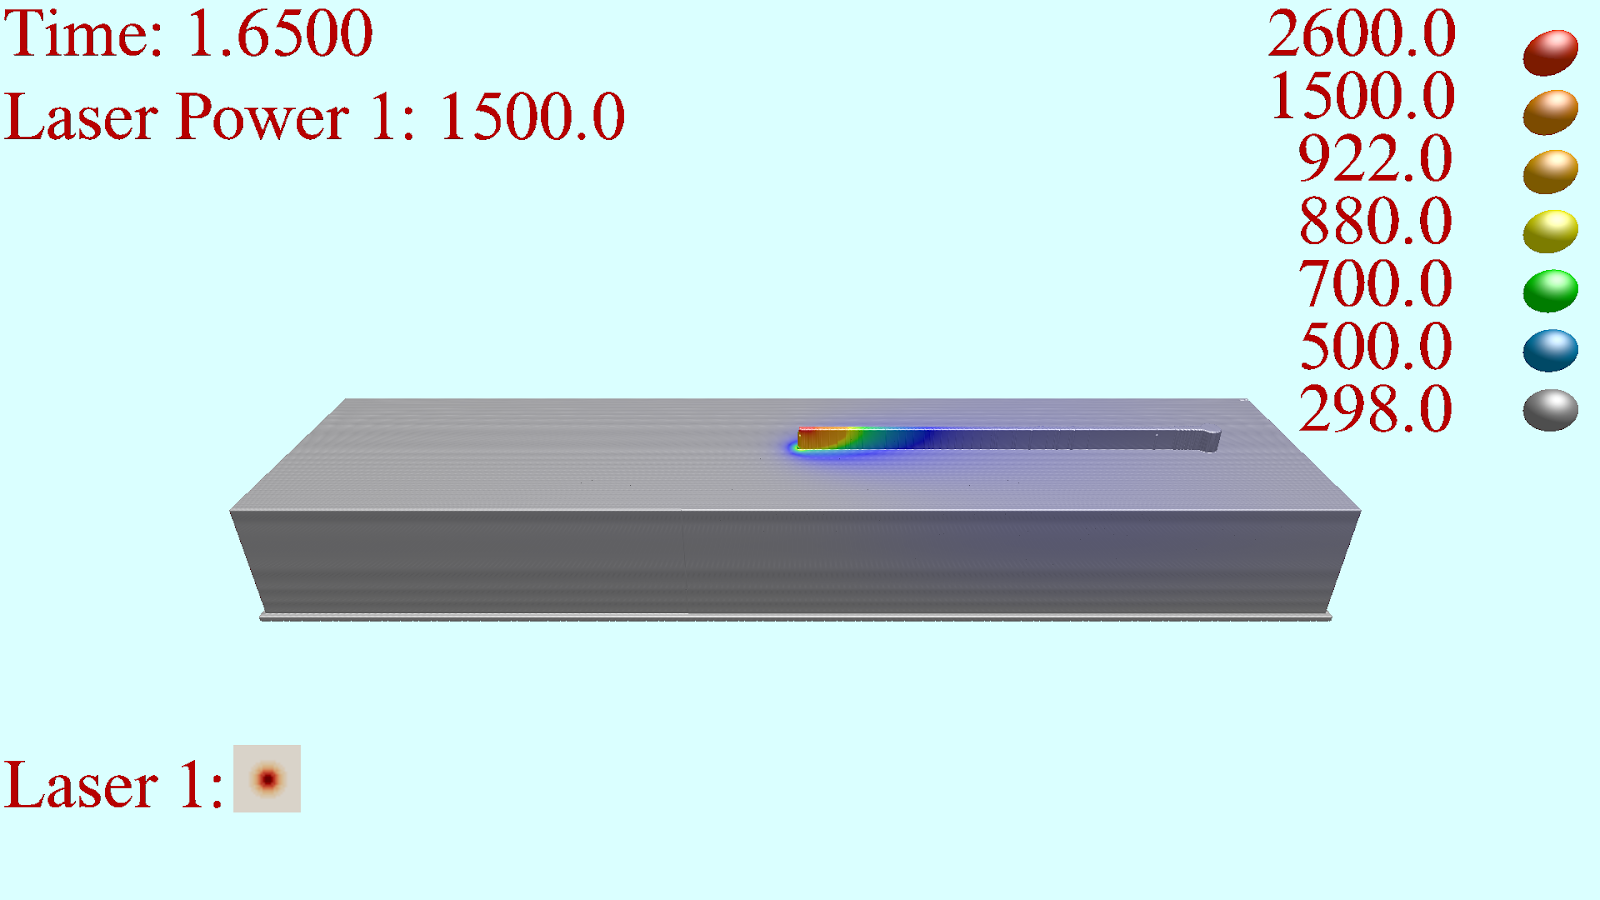
\includegraphics[width=\textwidth]{TEMP}
\caption{\centering \label{1a}}
\end{subfigure}
\begin{subfigure}[c]{0.3\textwidth}
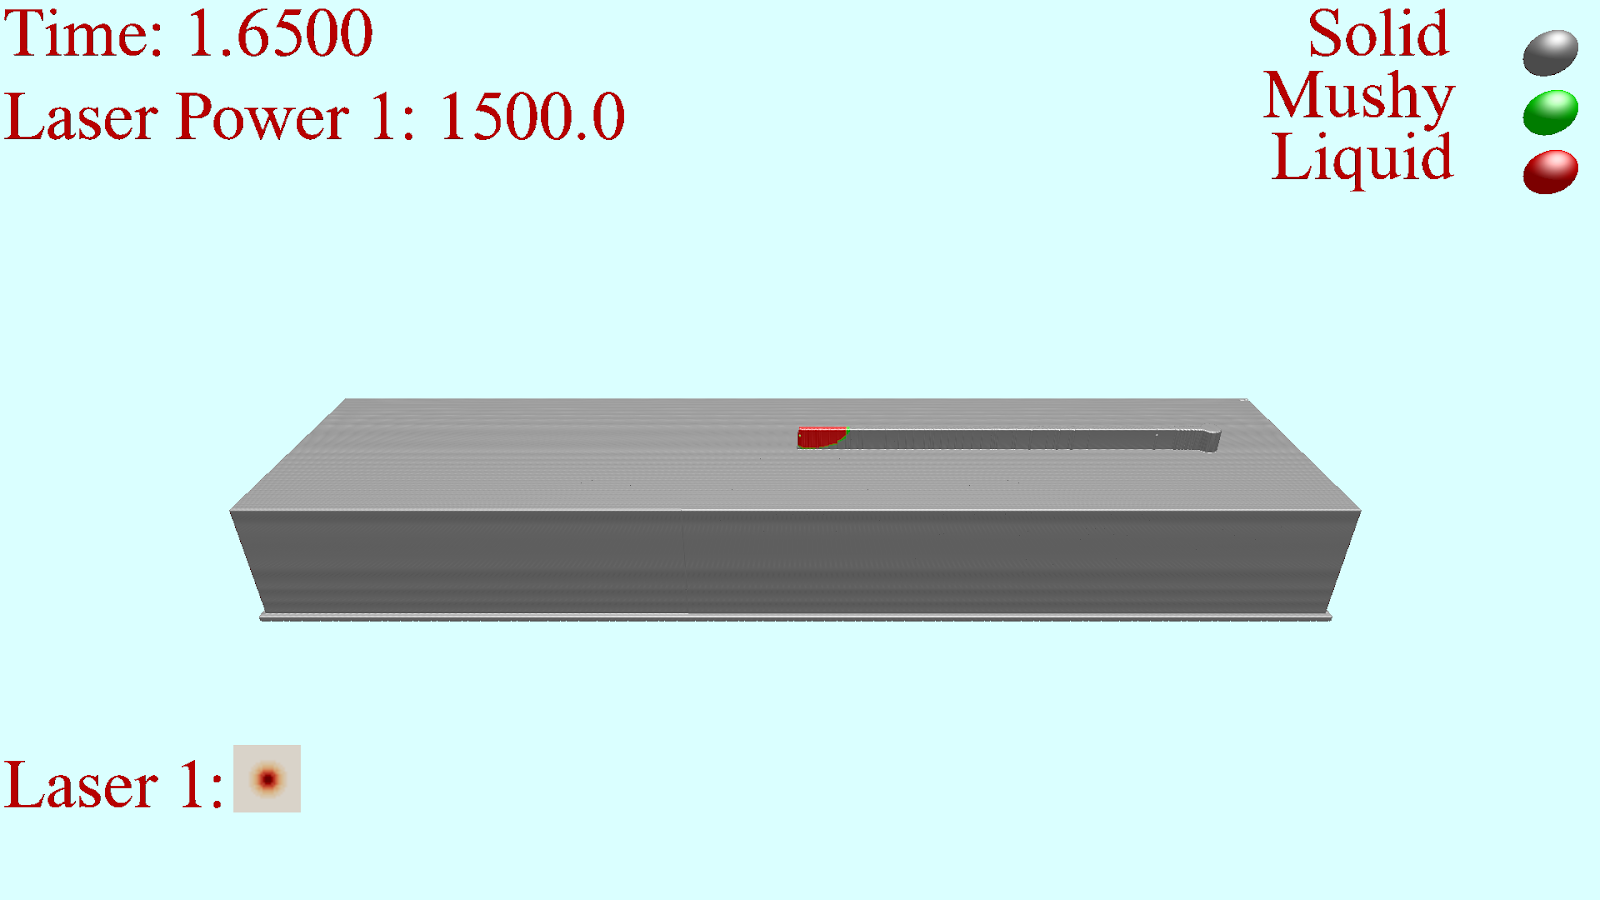
\includegraphics[width=\textwidth]{PHASE}
\caption{\centering }
\end{subfigure}
\begin{subfigure}[c]{0.3\textwidth}
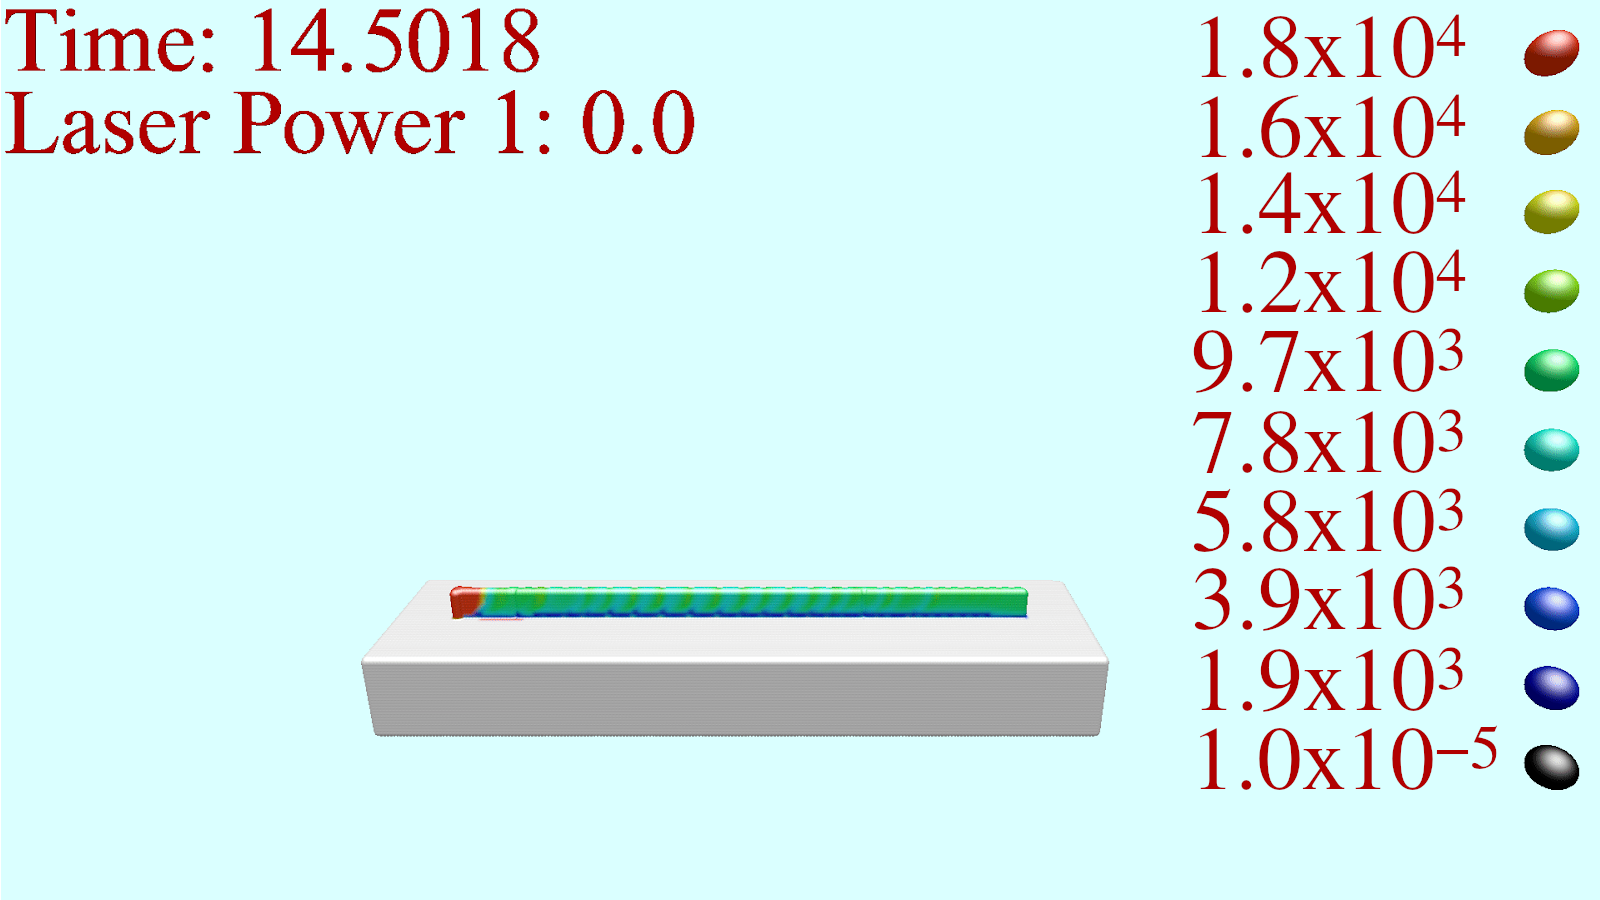
\includegraphics[width=\textwidth]{COOLRATE}
\caption{\centering }
\end{subfigure}
\caption{\hl{Examples} %MDPI: Please change the terms into scientific notation in the figure. (e.g., "$8 \times 10^{3}$", not "8e3"); Please change the hyphen (-) into minus sign ($-$, "U+2212"). e.g., "-1" should be "$-$1".
% This has been corrected
of data maps which can be expected from the simulation. \hl{(\textbf{a}) Temperature 
profile; (\textbf{b}) phase map; (\textbf{c}) cooling rate map.} %MDPI: please confirm we 
%moved subcaptions into captions; highlight below same as this
% These are correct
}
\label{fig:data_maps}	
\end{figure}

\clearpage 
Additionally, the laser in the simulation is modeled in 3D to be able to take into account 
the beam quality using the \ac{BPP} reported by the manufacturer and shown in Equation 
\eqref{eqn:bpp}, where $\theta$ and $w_0$ are the divergence angle and the beam waist 
respectively.
%MDPI: please confirm if format of BPP should be unified
% This looks correct in its current form
\begin{equation}\label{eqn:bpp}
	BPP = 0.5 \theta w_0
\end{equation} 
\hl{Lastly}, the model includes true ray tracing, enabling shadowing of the laser, the 
ability to define a mass that represents the machine acting as a heat sink during the build 
process, and the inclusion of temperature-dependent material properties.
% this is another instance of an equation breaking up a paragraph, please typeset however the editor deem appropriate


The main objective of the model is to accurately predict the thermal history of the build.  
To initially validate the models, the well-characterized and published material Ti-64 was 
used.  The validation was performed by scanning a laser on the surface of a substrate at 
three energy densities with the experimental parameters found in Table 
\ref{tab:ti64_parameters}, and the material properties used in the simulations can be seen 
in Table \ref{tab:ti64_properties}.

\begin{table}[H]
\caption{\hl{Simulation} %MDPI: please confirm we removed vertical lines of tables
%These look correct
 parameters used in Ti-64 validation.}
\label{tab:ti64_parameters}
\newcolumntype{C}{>{\centering\arraybackslash}X}
\begin{tabularx}{\textwidth}{CC}
\toprule
\textbf{Parameter} & \textbf{Value} \\ \midrule
Resolution & 60 $\upmu$m \\ \midrule
Laser diameter & 2.0 mm \\ \midrule
Laser Profile & TEM00 \\ \midrule
Laser power & 1000 W \\ \midrule
Energy density (Equation \eqref{eqn:eng_density}) & 13, 18, 24 $\frac{\text{W}}{\text{mm}^3/\text{s}}$ \\ \midrule
Scan Length & 45 mm \\ \midrule
Substrate dimensions & 55 mm \hl{$\times$} %MDPI: We revised the "x" into a multiplication sign ("\times" U+00D7). Please confirm.
%Confirmed
12.7 mm \hl{$\times$} 6.35 mm \\ 
\bottomrule
\end{tabularx}
\end{table}

\vspace{-12pt}
\begin{table}[H]
\caption{Ti-64 material properties used in validation.}
\label{tab:ti64_properties}
\newcolumntype{C}{>{\centering\arraybackslash}X}
\begin{tabularx}{\textwidth}{CCC}
\toprule
\textbf{Material Property} & \textbf{Value} & \textbf{Reference} \\ \midrule
Solidus temperature & 1603~$^{\circ}$C & \cite{welschgerhard_1993} \\ \midrule
Liquidus temperature & 1650~$^{\circ}$C & \cite{mills_2002} \\ \midrule
Solid density & 4420.0 $\frac{\text{kg}}{\text{m}^3}$ & \cite{mills_2002} \\ \midrule
Fluid density & 3920.0 $\frac{\text{kg}}{\text{m}^3}$ & \cite{mills_2002} \\ \midrule
Specific heat &  0.4--1.15 $\frac{\text{J}}{\text{gK}}$ & \cite{boivineau_2006} \\ \midrule
Thermal conductivity & 5.0--43.0 $\frac{\text{W}}{\text{mK}}$ &~\cite{boivineau_2006} \\ \midrule
Absorptivity & 0.4 &~\cite{fan_2012} \\ 
\bottomrule
\end{tabularx}
\end{table}


There are several representations of the energy density of a laser beam in \ac{AM}, but the 
most appropriate method of calculating the energy for the \ac{DED} process is to use the  
surface energy density, Equation \eqref{eqn:eng_density}, where \hl{$P$} is laser power, 
\hl{$A$} is the laser spot area, and \hl{$v$} is the scan 
speed~\cite{kurzynowskiEffectScanningSupport2019}.
% Updated to match the formatting of the equations
\begin{equation}
	SED_{area} = \frac{P}{A v} \label{eqn:eng_density}
\end{equation}


To analyze the results, the samples from the three different parameter sets were sectioned 
using a wire \ac{EDM}, polished using an automated polisher to a mirror finish, and 
etched using Kroll's reagent to make the melt track visible with an optical microscope, as 
can be seen in Figure \ref{fig:melt_track}a, this was performed at three points along the 
melt length.

\begin{figure}[H]
\begin{subfigure}{0.495\textwidth}
\includegraphics[width=\textwidth]{melt_track_image}
\caption{\centering}
\label{fig:melt_track_image}
\end{subfigure}
\begin{subfigure}{0.495\textwidth}
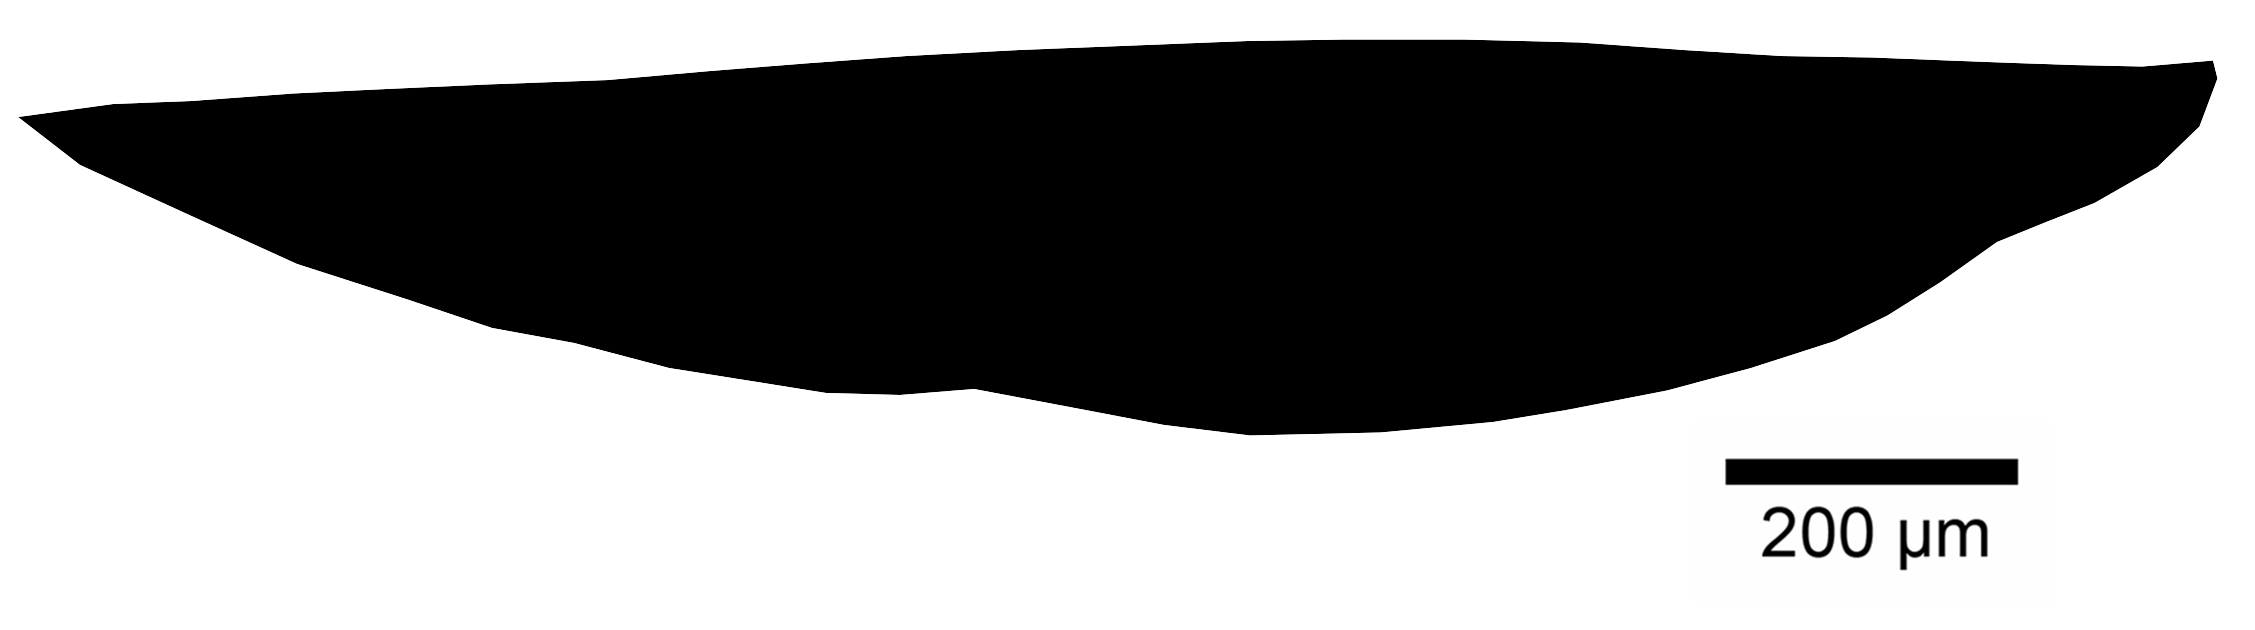
\includegraphics[width=\textwidth]{melt_track_bitmap}
\caption{\centering}
\label{fig:melt_track_bitmap}
\end{subfigure}
\caption{Analysis of sliced sample in Ti-64 validation. \hl{(\textbf{a}) Sample image of 
the etched slice; (\textbf{b}) melt pool extracted from etched slice.}}%MDPI: please comfirm
% confirmed
\label{fig:melt_track}
\end{figure}

The experiment and simulation were compared, and the resulting error for the width can 
be seen in Figure \ref{fig:ti64_melt_track}a and that of the depth can be seen in Figure 
\ref{fig:ti64_melt_track}b.

\begin{figure}[H]
\begin{subfigure}[c]{0.45\textwidth}
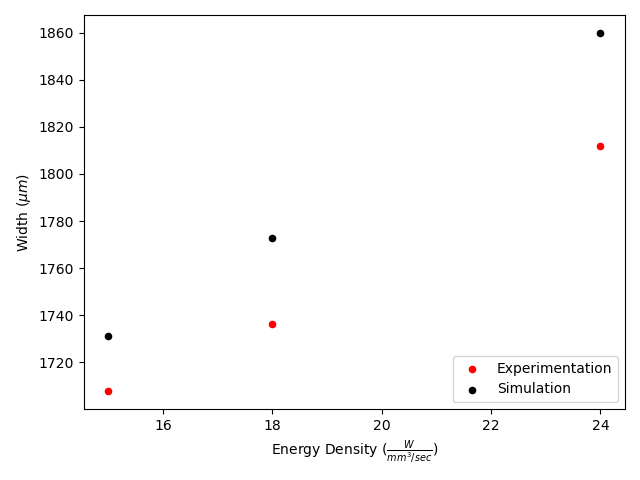
\includegraphics[width=\textwidth]{ti64_melt_track_width}
\caption{\centering}
\label{fig:ti64_melt_track_width}
\end{subfigure}
\begin{subfigure}[c]{0.45\textwidth}\centering
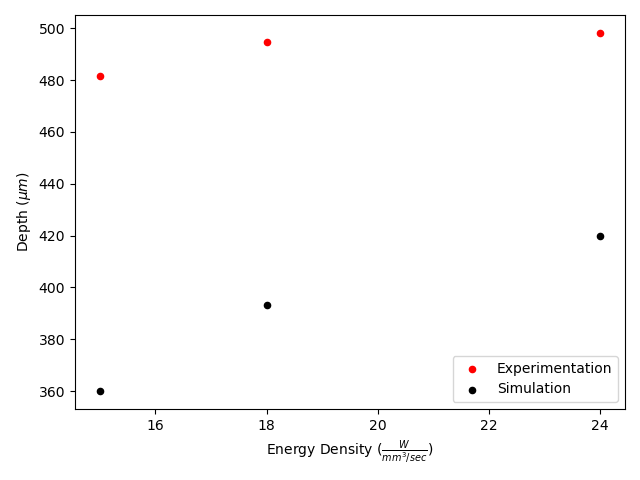
\includegraphics[width=\textwidth]{ti64_melt_track_depth}
\caption{\centering}
\label{fig:ti64_melt_track_depth}
\end{subfigure}
\caption{Comparison of simulation and experimentation in Ti-64 validation. \hl{(\textbf{a}) Width; (\textbf{b}) Depth.}}
% confirmed
\label{fig:ti64_melt_track}
\end{figure}
The average values that are reported on the graph have an associated standard deviation 
of 0.62 $\upmu$m, 13.7 $\upmu$m, and 7.74 $\upmu$m for the width measurements for 
the energy densities of 15 $\frac{\text{W}}{\text{mm}^3/\text{s}}$, 18 
$\frac{\text{W}}{\text{mm}^3/\text{s}}$, and 24 $\frac{\text{W}}{\text{mm}^3/\text{s}}$, 
respectively.  For the track depth, the standard deviations are 70.2 $\upmu$m, 113.7 
$\upmu$m, and 13.7 $\upmu$m for the energy densities of 15 
$\frac{\text{W}}{\text{mm}^3/\text{s}}$, 18~$\frac{\text{W}}{\text{mm}^3/\text{s}}$, and 
24 $\frac{\text{W}}{\text{mm}^3/\text{s}}$, respectively.

From the plots, it can be seen that the simulation is capable of predicting the width with an 
error of less than 3\%, and the depth error is between 15\% and 25\%.  The error in the 
width is very acceptable, at less than 3\%.
However, the error in the depth is larger due to the resolution (voxel size) of the 
simulation chosen and its size relative to the depth.  This error, of approximately 20\%, for 
the depths which range from 450--500 $\upmu$m is \mbox{1.3--1.7}~times the resolution, 
60 $\upmu$m, of the simulation.  Since the trends of the simulation and experimentation 
match and the error is within two resolution distances, the 20\% error in the depth is 
considered acceptable as well. 
This shows that the mathematical models developed are accurate and if the material property is well characterized, the simulation will produce accurate results.


\subsection{Search Algorithm Description}
\label{algrothim_description}

The search algorithm chosen was the Nelder--Mead search algorithm~\cite{nelder_1965}.  
This method was selected because it is one of the most popular direct search methods for 
the minimization of functions.  The Nelder--Mead approach is a local optimization search 
that does not rely on the knowledge of the gradient to select the next search point.  This is 
critical for the application of simulation results because the gradient is unknown and 
finding it would involve running a large number of simulations.  With simulation times 
that can reach into days long, this is a critical consideration.  
Instead of knowing the actual function, it relies on n~+~1 vertices.  This results in a smaller number of simulation runs being needed to perform the minimization~\cite{wang_2011}.
The flow chart in Figure \ref{fig:nm_flow} is the flow that is used to determine the next search point.

\begin{figure}[H]
	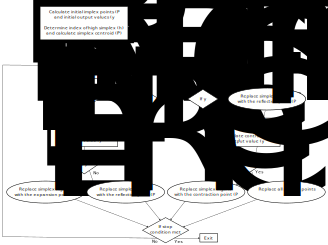
\includegraphics[width=\textwidth]{nm_flow}
	\caption{\hl{Flow} %MDPI: Please change the hyphen (-) into minus sign ($-$, "U+2212"). e.g., "-1" should be "$-$1".
	% If this is referring to the image, this has been done.  Otherwise, please advise where the hyphens are that need to be modified.
 chart for the Nelder--Mead search algorithm}
	\label{fig:nm_flow}
\end{figure}

The search begins by calculating the reflection point using Equation \eqref{eqn:reflection}, 
where $\alpha$ is the reflection coefficient.
	\begin{equation}\label{eqn:reflection}
		P_{refl} = (1 + \alpha) P_{cent} - \alpha P_{high}
	\end{equation}
\hl{If this} reflection point is smaller than the smallest current simplex value, then the expansion is calculated using Equation \eqref{eqn:expansion}, where $\gamma$ is the expansion coefficient.
	\begin{equation}\label{eqn:expansion}
		P_{exp} = \gamma P_{refl} - (1 - \gamma) P_{center}
	\end{equation}
\hl{If the} expansion point is smaller than the reflection point, then the expansion point is used to replace the largest simplex member.  Otherwise, if the reflection point is larger than the expansion point, the reflection point is used to replace the largest member of the simplex, and the algorithm is restarted.
If the reflection point is larger than the smallest simplex point and smaller than the 
second-largest point, then the highest point of the simplex is replaced with the reflection, 
and the algorithm is restarted. 
If the reflection point is between the simplex highest value and the second-highest value, a 
contraction is calculated, using Equation \eqref{eqn:reflection}, with the highest values 
being replaced with the reflection.  Otherwise, the contraction is calculated with the 
original simplex, still using Equation \eqref{eqn:reflection}, where $\beta$ is the 
contraction coefficient.
\begin{equation}
\label{eqn:contraction}
P_{cont} = \beta P_{high} - (1 - \beta) P_{cent}	
\end{equation}
\hl{If the} contraction point is smaller than the largest point of the simplex, then the 
contraction replaces the largest point and the algorithm is continued.
However, if the contraction point is larger than the highest point, a shrink step is performed, detailed in Equation \eqref{eqn:shrink}, where $\delta$ is the shrink coefficient and the algorithm is restarted.
\begin{equation}
\label{eqn:shrink}
P_{i} = \delta P_{i} + (1 - \delta) P_{low}
\end{equation}
% The authors are not sure why these are marked.  If it is due to the lack of indention, it is meant to be a single paragraph with 3 equations in it, however, LaTeX is not facilitating that.  The authors defer to the editors as to the best formatting for this paragraph


\subsection{Selection of Properties}
\label{sensetivity_results}

One of the attractive characteristics of the Nelder--Mead search algorithm is its ability to 
scale to an unlimited number of unknowns.  The main adverse effects of the scaling are the 
increased number of runs and the combination of the errors.  As the number of unknowns 
increases, the complexity of the search space increases, which in turn increases the number 
of iterations needed to find a minimum.  This can result in drastically longer wait times for 
the search results.  Additionally, with the increased number of unknowns, the stop 
condition of the search algorithm will be met at a different interval since the stop condition 
is based on the variance in the simplex.  This may result in modifications to the stop 
conditions being necessary as a larger number of unknowns are included.  If the response 
variable is properly defined, it will not affect the model's results if more unknowns are 
included~\cite{wang_2011}.

To reduce the complexity of the search algorithm, a sensitivity analysis was performed.
This work began by finding the material properties that were needed in the models, as 
summarized in Table \ref{tab:sens_properties}.


\begin{table}[H]
\caption{Key material properties in thermal modeling of AM.}
\label{tab:sens_properties}
%\newcolumntype{C}{>{\centering\arraybackslash}X}
\begin{tabularx}{\textwidth}{CC}
\toprule
\textbf{Material Property} & \textbf{\hl{References} %MDPI: please confirm we added ``s''
%confirmed
} \\ \midrule
Solidus temperature & \cite{joseph_r_davis_aluminum_2001, lundberg_material_1994, ulbrich_wire_2014, matweb}\\
\midrule
Liquidus temperature & \cite{joseph_r_davis_aluminum_2001, lundberg_material_1994, ulbrich_wire_2014, matweb}\\
\midrule
Solid density & \cite{matweb, amesweb}\\
\midrule
Fluid density & \cite{matweb, schmitz_density_2012, leitner_thermophysical_2017}\\
\midrule
Specific heat & \cite{lundberg_material_1994, leitner_thermophysical_2017}\\
\midrule
Thermal conductivity & \cite{lundberg_material_1994, leitner_thermophysical_2017}\\
\midrule
Absorptivity & \cite{funck_tailored_2014, boyden_temperature_2006, el-hameed_anodic_2017}\\
\bottomrule
\end{tabularx}
\end{table}

These properties were varied according to a Placket--Burman design experiment to 
determine the properties which, when changed, had a statically significant effect on the 
resulting melt pool width, depth, and volume, as measured in Figure \ref{fig:slices}.

\begin{figure}[H]
\begin{subfigure}[t]{0.22\textwidth}
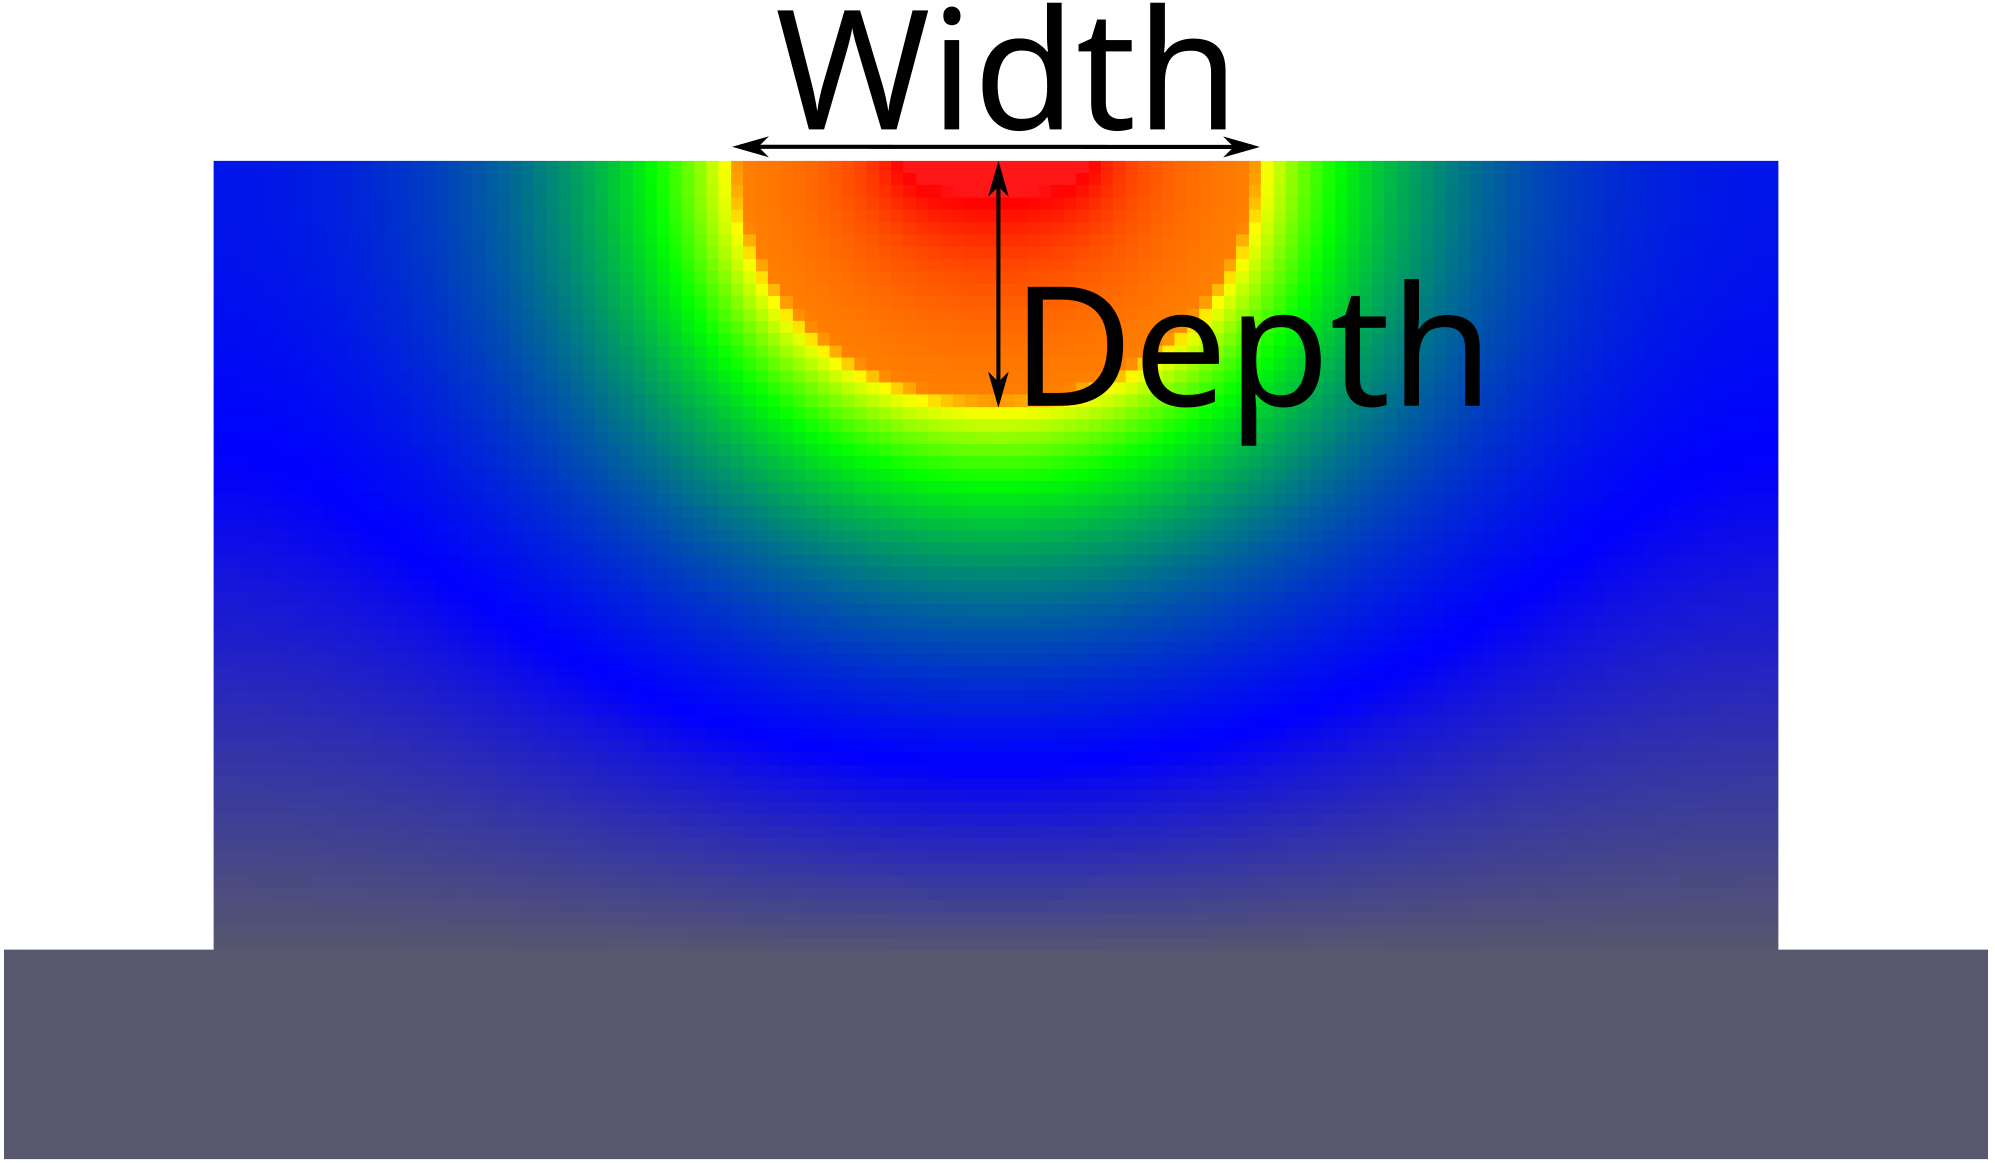
\includegraphics[height=0.6in]{slice_y_annotated}
\caption{\centering}
\label{fig:slice_y_annotated}
\end{subfigure}
\begin{subfigure}[t]{0.77\textwidth}
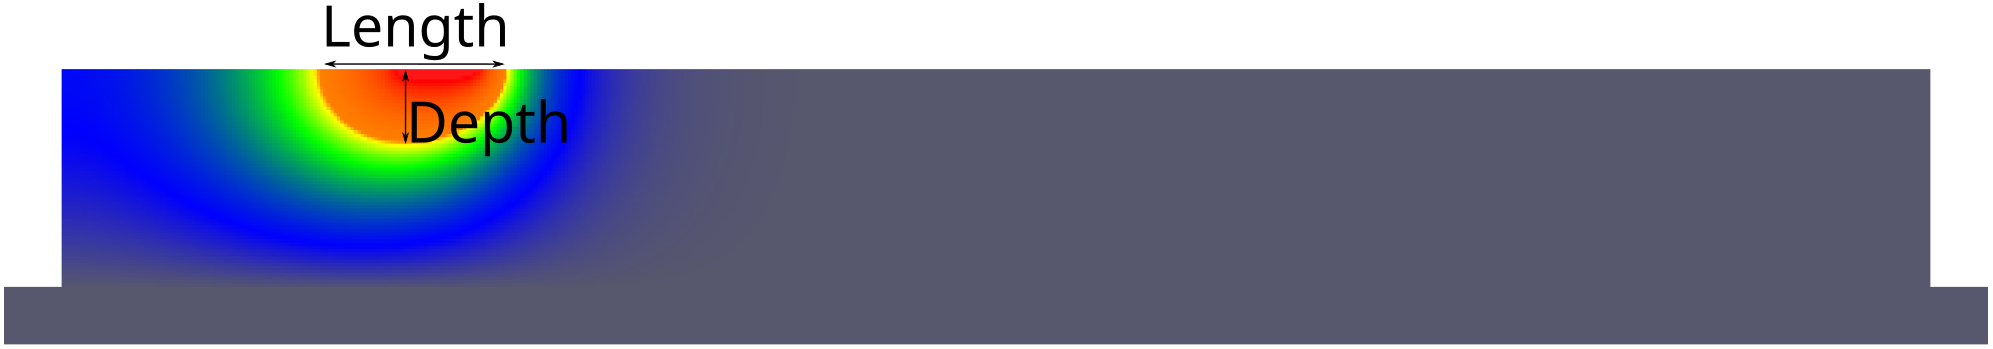
\includegraphics[height=0.6in]{slice_x_annotated}
\caption{\centering}
\label{fig:slice_x_annotated}
\end{subfigure}
\caption{Example measurements of the melt pool. \hl{(\textbf{a}) Width; (\textbf{b}) 
length.}}
%confirmed subcaptions
\label{fig:slices}
\end{figure}

Analyzing these results with Pareto charts of the standardized effects of the variables and partial regression plots of the residuals it was determined that the variables in Table \ref{tab:crit_mat_prop} had a statically significant effect on the resulting melt track when modified.

\begin{table}[H]
\caption{\hl{Critical} %MDPI: please confirm there is no table header
%confirmed
 material properties.}
\label{tab:crit_mat_prop}
\begin{tabularx}{\textwidth}{C}
\toprule
Laser absorption at 880~$^{\circ}$C \\ \midrule
Laser absorption at 922~$^{\circ}$C \\ \midrule
Thermal conductivity at 922~$^{\circ}$C \\ \midrule
Thermal conductivity at 1491~$^{\circ}$C \\ \midrule
Specific heat at 733~$^{\circ}$C \\ 
\bottomrule			
\end{tabularx}
\end{table}

This work included the laser diameter in the search algorithms dataset due to the difficulty associated with accurately measuring the diameter, this process is detailed in~\cite{floodSensitivityAnalysisDirected2023}.



\subsection{Parameter Search and Simulation Setup}
\label{sim_setup}

For this study, the Nelder--Mead search algorithm parameters that were used can be seen 
in Table \ref{tab:nm_parameters}.

\begin{table}[H]
\caption{Nelder--Mead algorithm parameters.}
\label{tab:nm_parameters}
\begin{tabularx}{\textwidth}{CC}
\toprule
\textbf{Parameter} & \textbf{Value} \\ \midrule
$\alpha$ & 5.0 \\ \midrule
$\gamma$ & 10.0 \\ \midrule
$\beta$ & 0.5 \\ \midrule
$\sigma$ & 0.5 \\ 
\bottomrule
\end{tabularx}
\end{table}
These parameters were chosen because they fell within the guidelines of the algorithm 
description and after trial and error produced the most efficient 
searching~\cite{nelder_1965}.

The initial parameter values that were used as the starting point for the search algorithm 
can be seen in Table \ref{tab:starting_mat_prop_complete}.  These values were chosen 
based on the values that were found in the literature for similar aluminum alloys.  The 
laser diameter was chosen based on the measuring of a melt track width on a substrate. 

\begin{table}[H]
\caption{Generic aluminum material properties found in the literature.}
\label{tab:starting_mat_prop_complete}
\begin{tabularx}{\textwidth}{cCCC}
\toprule
\textbf{Property} & \textbf{Material Temp.} & \textbf{Value} & \textbf{Ref.} \\ \midrule
Laser absorption & 880~$^{\circ}$C & 15.0\% &~\cite{boyden_temperature_2006} \\ \midrule
Laser absorption & 922~$^{\circ}$C & 30.0\% &~\cite{boyden_temperature_2006} \\ \midrule
Thermal conductivity & 922~$^{\circ}$C & 88.8 $\frac{\text{W}}{\text{mK}}$ &~\cite{leitner_thermophysical_2017}\\ \midrule
Thermal conductivity & 1491~$^{\circ}$C & 104.9 $\frac{\text{W}}{\text{mK}}$ &~\cite{leitner_thermophysical_2017}\\ \midrule
Specific heat & 733~$^{\circ}$C & 1108.0 $\frac{\text{J}}{\text{kgK}}$ &~\cite{leitner_thermophysical_2017}\\ \midrule
Laser diameter & & 1.6 mm & \\ 
\bottomrule
\end{tabularx}
\end{table}

To ensure the search algorithm did not waste time searching in unacceptable regions, the 
constraint was included that none of the material properties were allowed to become 
negative.  This was the only constraint that was needed in addition to the inherent 
constraints of the Nelder--Mead algorithm.

The experimental setup that was used was a simple laser scanning of the surface of a 
substrate, as shown in Figure \ref{fig:melt_validation_example}, with the parameters 
shown in Table \ref{tab:exp_constants}.  This was chosen to simplify the experiment.  This 
setup removes the complexity associated with adding material, which includes the rate of 
material addition, molten metal flow parameters, and acceleration effect associated with 
turning during deposits.

\begin{figure}[H]
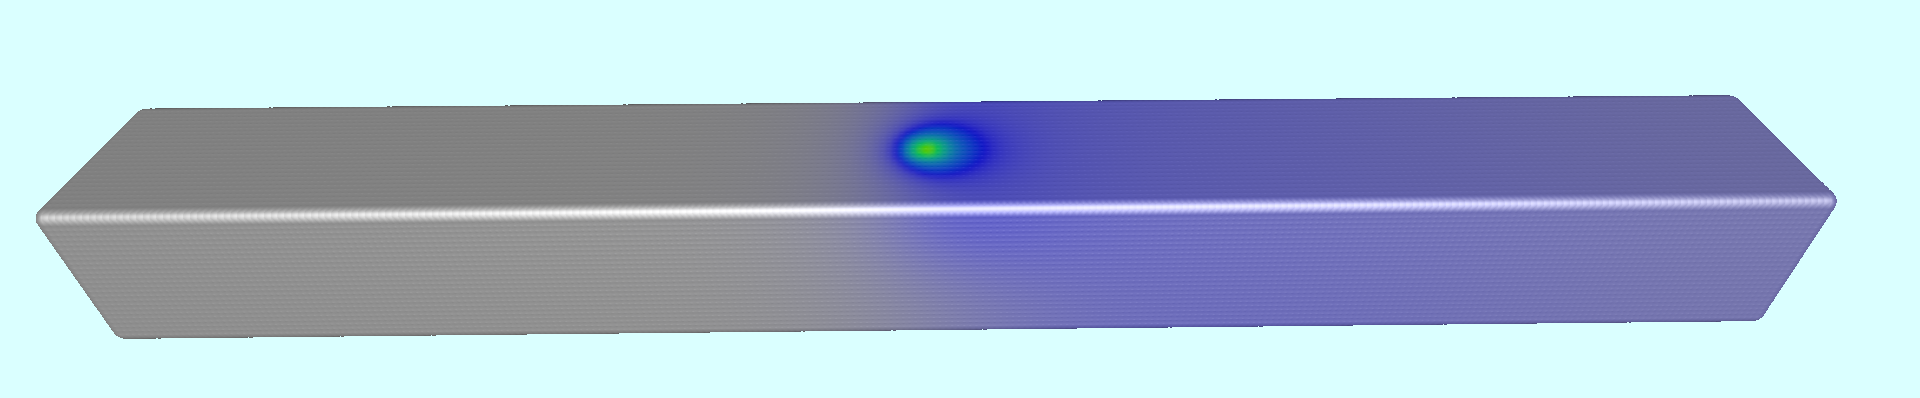
\includegraphics[width=0.75\textwidth]{melt_validation_example}
\caption{Example of simulation setup used to determine melt track size.}
\label{fig:melt_validation_example}
\end{figure}

\begin{table}[H]
\caption{Experimental constants used in search algorithm experiments.}
\label{tab:exp_constants}
\begin{tabularx}{\textwidth}{LL}
\toprule
\textbf{Parameter} & \textbf{Value} \\ \midrule
Resolution (voxel size) & 100 $\upmu$m \\ \midrule
Laser Power & 1750 W \\ \midrule
Laser Scan Speed & 1143 mm/min \\ \midrule
Laser Profile & Top Hat \\ \midrule
Scan Length & 77 mm \\ \midrule
Substrate dimensions & 82 mm $\times$ 8 mm $\times$ 8 mm \\ 
\bottomrule
\end{tabularx}
\end{table}



\subsection{Simulation Analysis}
\label{sim_analysis}

Upon completion of each simulation run, the saved data files were analyzed to determine 
the regions of the simulation that had melted.  This was performed by developing a map 
that marked the locations of the domain that had ever been in the fluid phase.  This map 
was then used to determine the width and depth of the melt track along the scan length, 
excluding the beginning and end, where effects from starting and stopping motion would 
affect the results.  These width and depth measurements along the scan length were 
averaged to develop a single measurement that could be compared to the 
experimentation.  

The experimental results were similarly determined; however, instead of a continuous set 
of measurements, there were four discrete measurements.  These were obtained by slicing 
the substrate at the prescribed locations using a wire \ac{EDM}.  These slices were 
polished using an automatic polishing machine up to a mirror finish and etched using 
Keller's reagent to make the microstructural differences visible by an optical microscope; 
an example of this can be seen in Figure \ref{fig:7075_7_8C}, where the dark region had 
been melted during the experimentation.

\begin{figure}[H]
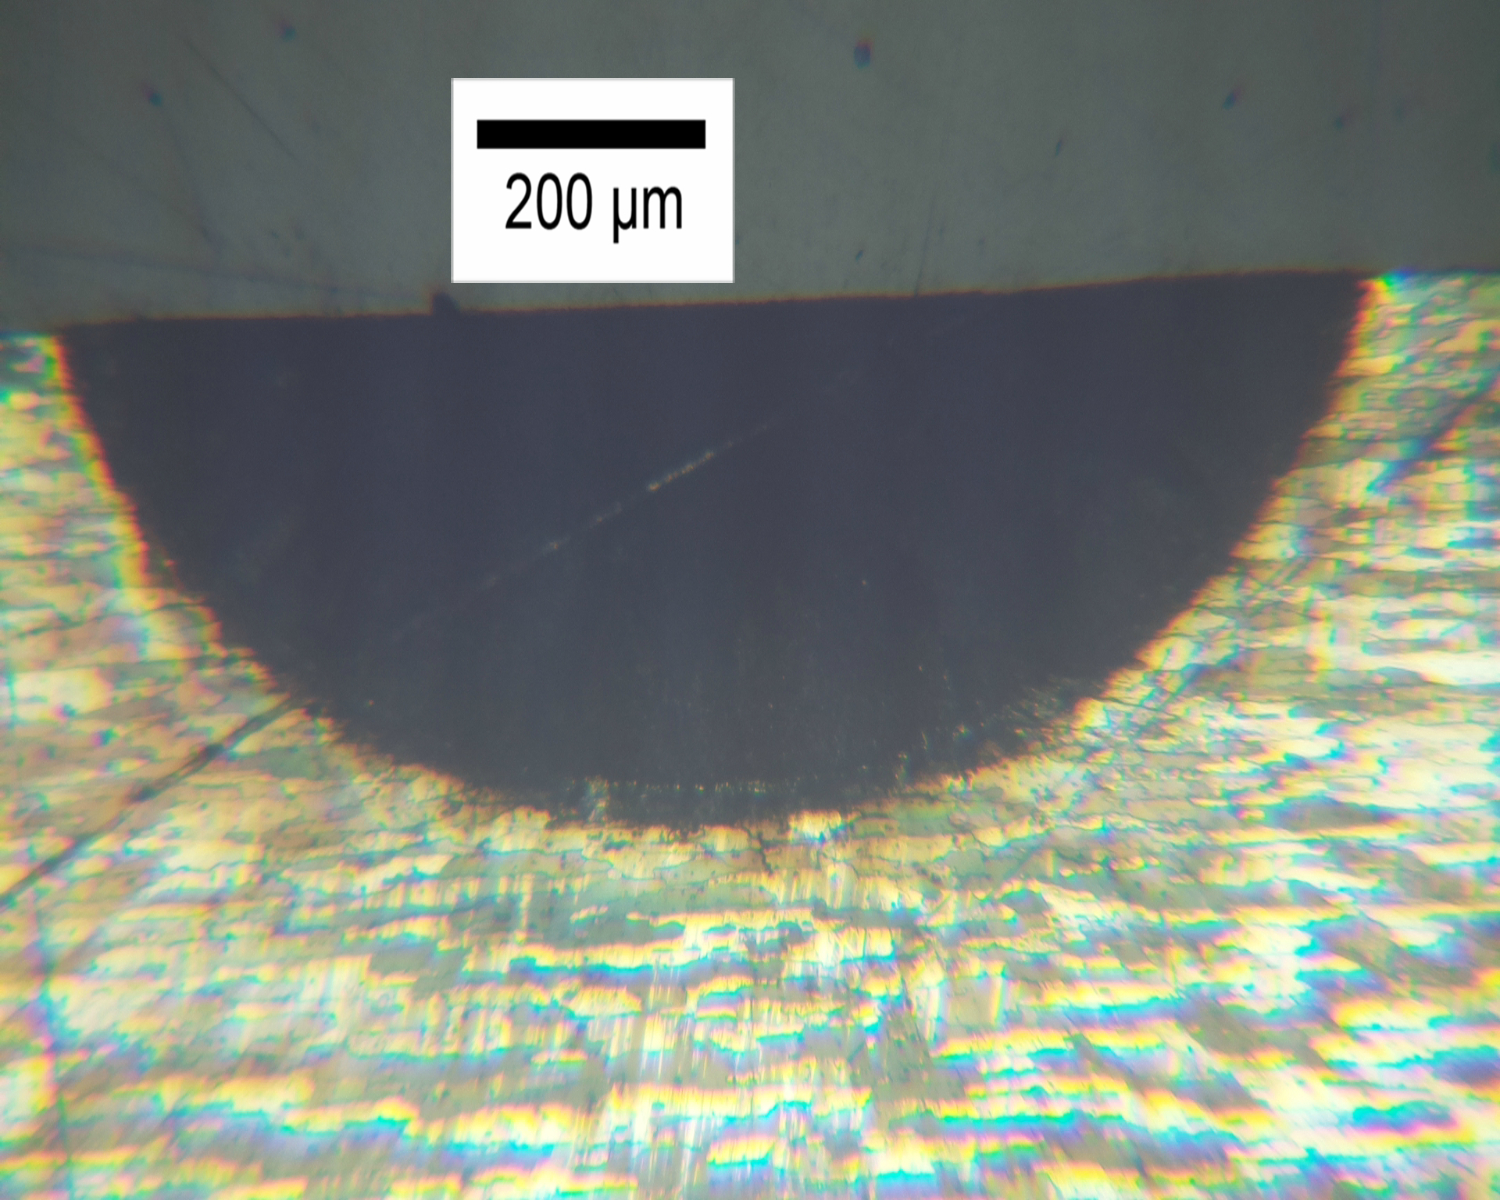
\includegraphics[width=0.5\textwidth]{7075_7_8C}
\caption{Example of sliced, polished, and etched slice from aluminum experimentation}
\label{fig:7075_7_8C}
\end{figure}

For the Nelder--Mead search to function properly, a response variable needed to be 
defined.  This function needed to characterize the accuracy of the simulation into a single 
parameter which could be minimized and upon minimization would result in the most 
accurate simulation.  To accomplish this goal, Equation \eqref{eqn:response} was 
developed.  This equation takes into account the error in the width of the simulation along 
with the error in the depth.  This equation results in a non-negative number where 0 
represents a simulation that perfectly matched \hl{experimentation.} %MDPI: please 
%confirm if * in equations should be multiplication sign $\times$
%confirmed
\begin{equation}\label{eqn:response}
	\begin{split}
		Response =  \Biggl ( &\frac{\lvert Sim.\ Width - Exp.\ Width \rvert}{Exp.\ Width} + \\ 
		&\frac{\lvert Sim.\ Depth - Exp.\ Depth \rvert}{Exp.\ Depth} \Biggr ) \times 100
	\end{split}
\end{equation}



\section{Results}
\subsection{Search Algorithm Results}
\label{results}

The search algorithm was allowed to search the space to determine the best material 
properties.  The resulting response variables can be found in Figure 
\ref{fig:response_complete}, where the blue circular markers indicate material datasets 
that developed a melt track and the red diamond markers did not have the energy density 
to produce a melt track.

\begin{figure}[H]
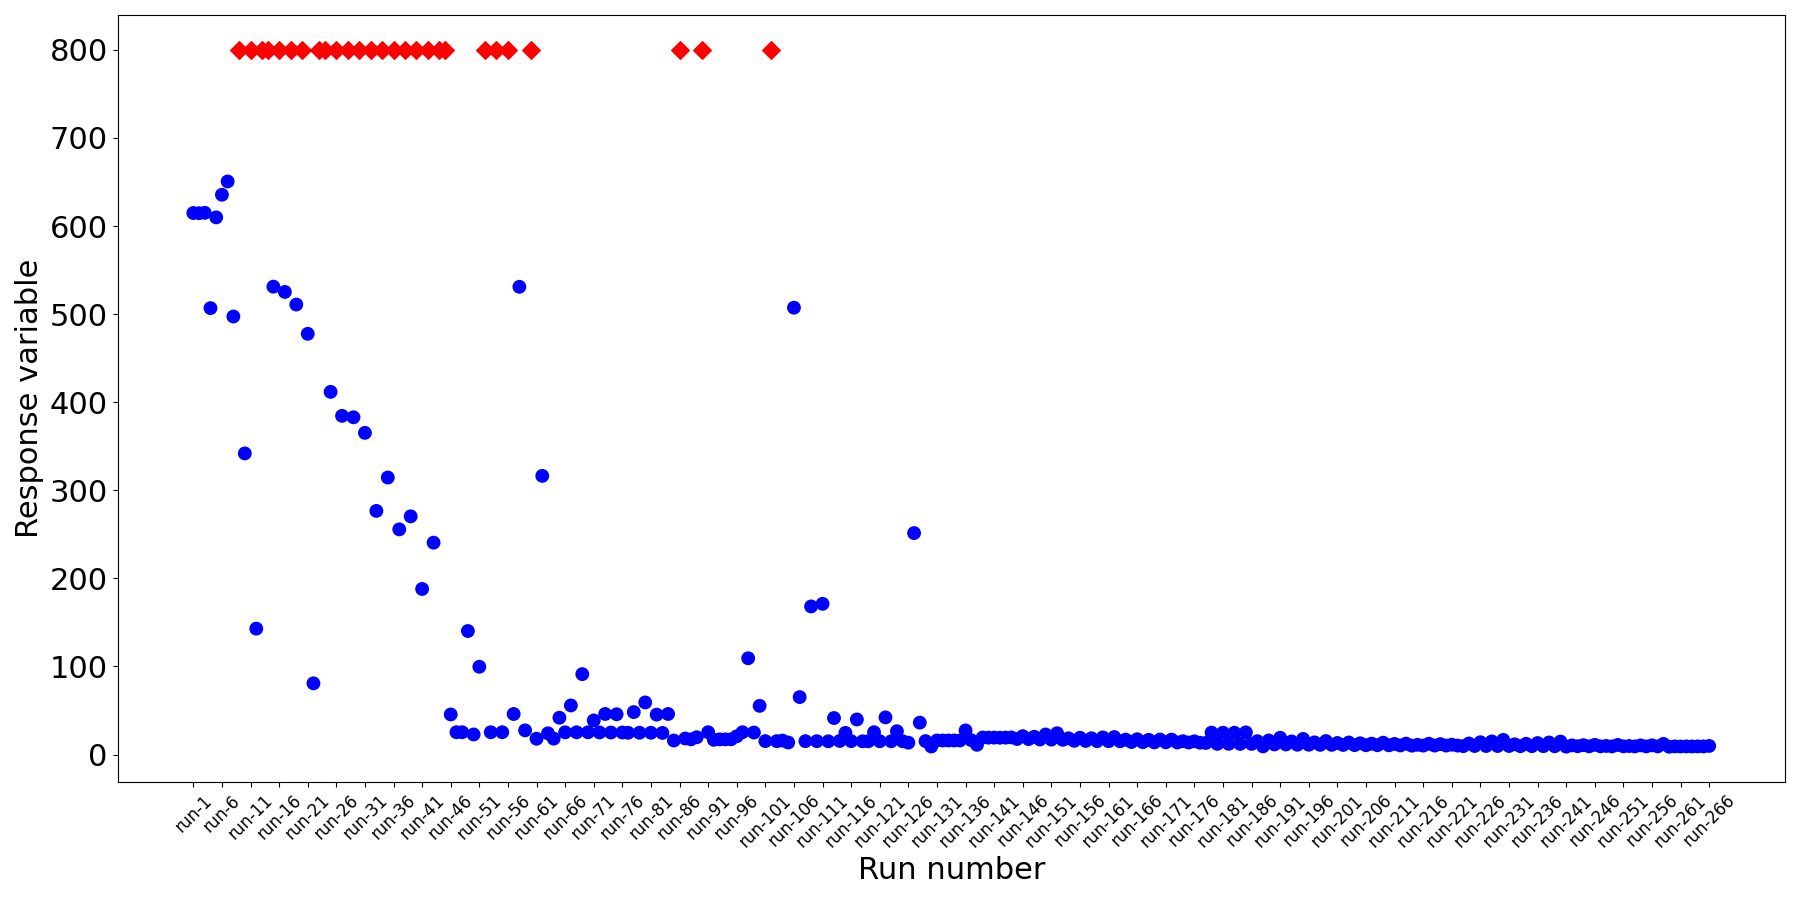
\includegraphics[width=0.75\textwidth]{response_complete}
\caption{\hl{Response variable} of the search algorithm for material properties and laser 
diameter, where the blue circle marks developed a melt track and the red diamonds did 
not.}%MDPI: Please confirm different color whether need add explanation, same as figure 9
% This is complete, Figure 9 has slightly different markers, this caption is correct
\label{fig:response_complete}
\end{figure}

Due to the vast difference in scale of the initial responses and the final response variables, 
a new plot, Figure \ref{fig:response_zoomed}, was created, which has a max Y value of just over 30.  In this plot, the blue 
circular markers have a response variable less than 30, the green triangle markers are those 
that completed with a melt track but had response variables greater than 30, and the red 
diamond markers are those that did not produce a melt track.

\begin{figure}[H]
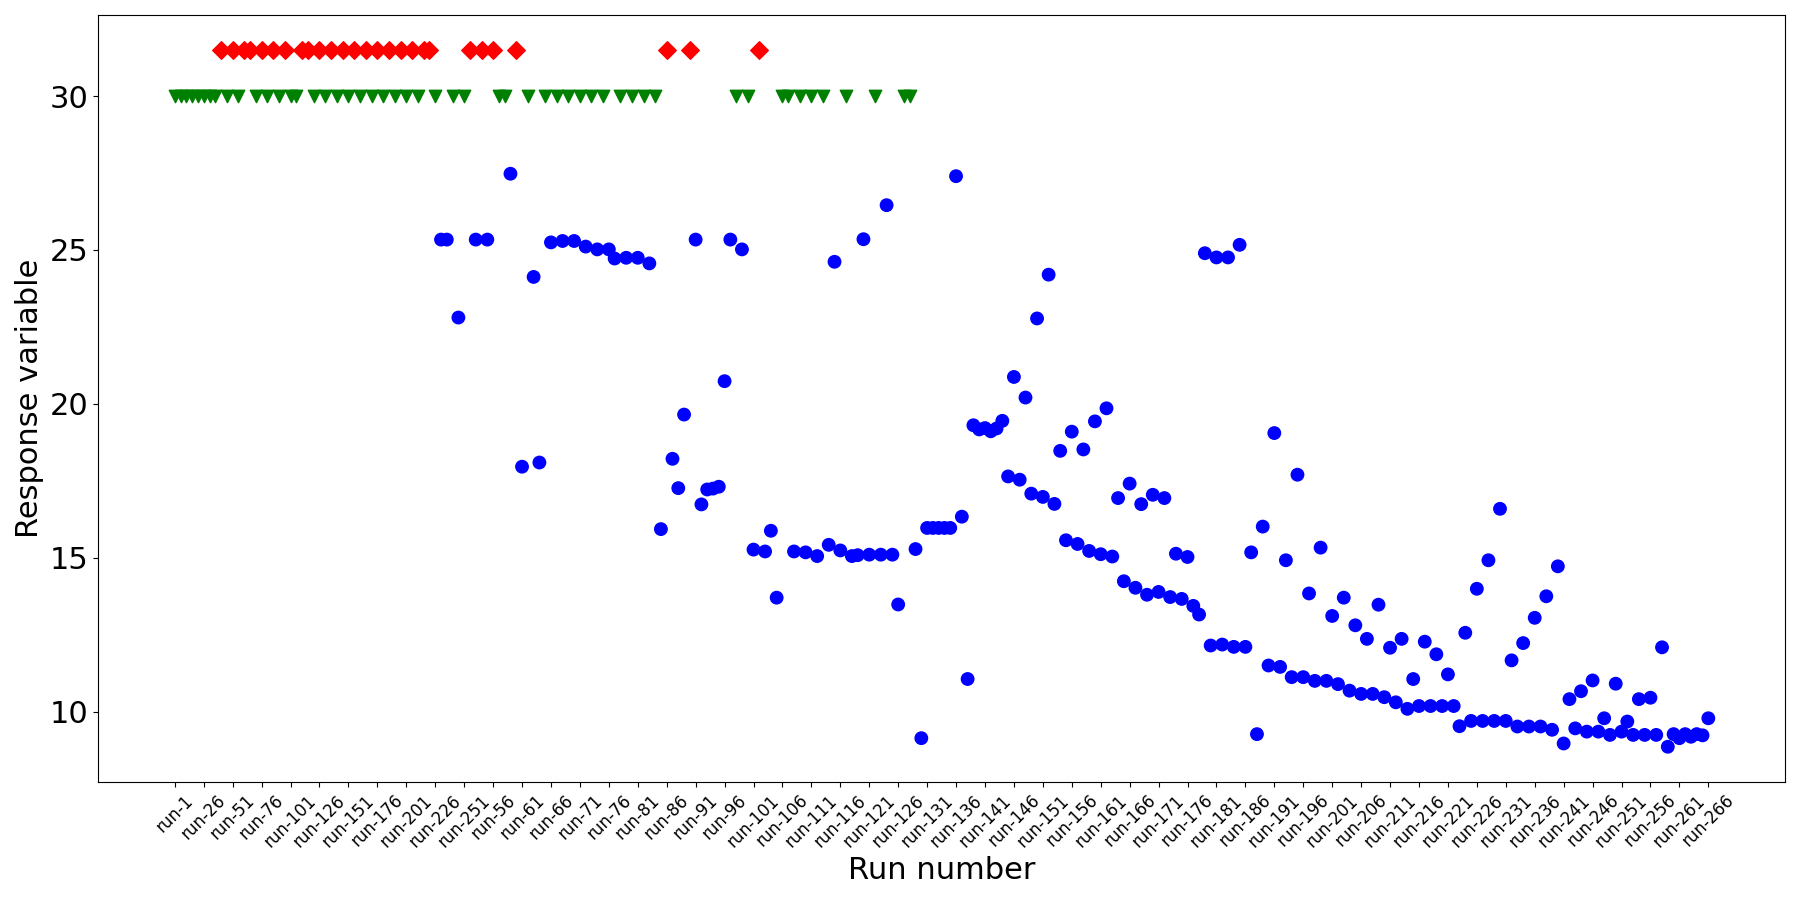
\includegraphics[width=0.75\textwidth]{response_zoomed}
\caption{\hl{Response} %MDPI: Please cite the figure in the text and ensure the first citation of each figure appears in numerical order.
% Added in line 753
 variable of the search algorithm for material properties and laser diameter with max y axis value of 30 where the blue circle marks developed a melt track, green triangles developed a melt pool but had a response greater than 30, and red diamonds did not develop a melt pool.}
\label{fig:response_zoomed}
\end{figure}

In addition to these plots, the error in the width and depth were plotted and can be seen in 
Figure \ref{fig:tuning_error_complete}.  In these plots, it can be seen that the error in the 
width is 8.83\% and the error in the depth is 0.03\%.  It is not fully understood why all the 
error is coming from the width; however, it is theorized that this is a product of the 
difference in the size of the width vs. the depth, since the width is nearly triple that of the 
depth.

\begin{figure}[H]
\begin{subfigure}[c]{0.475\textwidth}
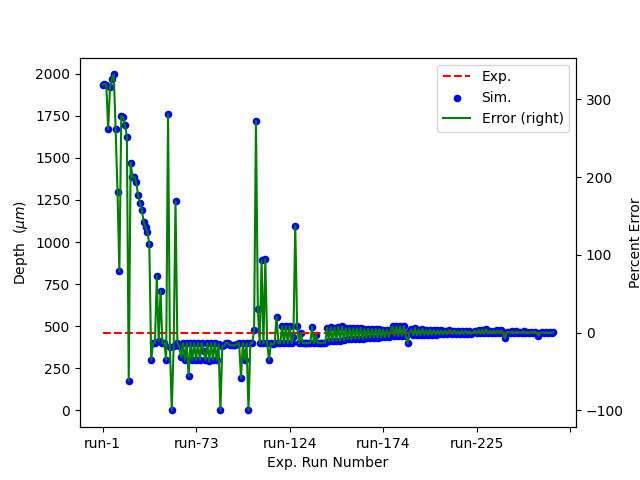
\includegraphics[width=\textwidth]{tuning_error_depth_complete}
\caption{\centering}
\label{fig:tuning_error_depth_complete}
\end{subfigure}
\begin{subfigure}[c]{0.475\textwidth}
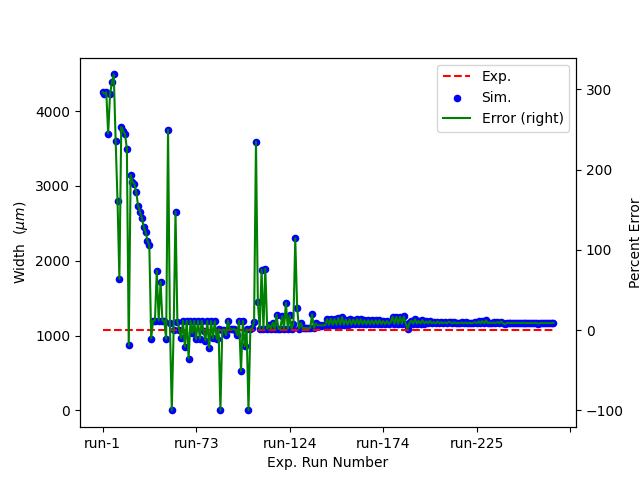
\includegraphics[width=\textwidth]{tuning_error_width_complete}
\caption{\centering}
\label{fig:tuning_error_width_complete}
\end{subfigure}
\caption{Error in the individual runs of the simulations during the search algorithm. 
\hl{(\textbf{a}) Melt track depth; (\textbf{b}) melt track width.}}
% confirmed
\label{fig:tuning_error_complete}
\end{figure}

The search algorithm completed and reduced the combined error from over 600\% when 
starting from the material properties found in the literature for the generic aluminum 
material properties, found in Table \ref{tab:starting_mat_prop_complete}, to 9.1\% when 
using the values found in Table \ref{tab:7000_mat_prop_complete}.

\begin{table}[H]
\caption{Optimized aluminum material properties and laser diameter dataset for the 
developed simulation.}
\label{tab:7000_mat_prop_complete}
\begin{tabularx}{\textwidth}{CCC}
\toprule
\textbf{Property} & \textbf{Material Temp.} & \textbf{Value} \\ \midrule
Laser absorption & 880~$^{\circ}$C & 16.8\% \\ \midrule
Laser absorption & 922~$^{\circ}$C & 10.0\%\\ \midrule
Thermal conductivity & 922~$^{\circ}$C & 32.2 $\frac{\text{W}}{\text{mK}}$\\ \midrule
Thermal conductivity & 1491~$^{\circ}$C & 152.3 $\frac{\text{W}}{\text{mK}}$\\ \midrule
Specific heat & 733~$^{\circ}$C & 2957.6 $\frac{\text{J}}{\text{kgK}}$ \\ \midrule
Laser diameter & & 0.864 mm \\ 
\bottomrule
\end{tabularx}
\end{table}

\subsection{Search Results Validation}
\label{validation}

To ensure that the search algorithm results were valid across laser travel speeds and 
power levels, a range of eight other parameters were compared with the experimental 
results.
These experiments and simulations were set up and analyzed in the same manner as the 
search algorithm experimental setup.  The base experimental parameters can be seen in 
Table \ref{tab:exp_constants}, with the scan speed and laser power being varied as seen in 
Table \ref{tab:val_parameters} and the simulation material properties were used from 
Table \ref{tab:7000_mat_prop_complete}.

\begin{table}[H]
\caption{Laser processing parameters validation processing parameters.}
\label{tab:val_parameters}
\begin{tabularx}{\textwidth}{CCC}
\toprule 
\textbf{Exp. Id.} & \textbf{Scan Speed (mm/min)} & \textbf{Laser Power (W)} \\ \midrule
1 & 762 & 1000 \\ \midrule 
2 & 762 & 1500 \\ \midrule 
3 & 762 & 1250 \\ \midrule  
4 & 1143 & 1250 \\ \midrule 
5 & 1143 & 1500 \\ \midrule
6 & 1524 & 1750 \\ \midrule  
7 & 1524 & 1500 \\ \midrule  
8 & 1524 & 2000 \\ 
\bottomrule  
\end{tabularx}
\end{table}

These speeds and powers were first completed with the literature-determined values in 
Table \ref{tab:starting_mat_prop_complete}, and the results can be seen in Figure 
\ref{fig:melt_track_val_baseline}.

\vspace{-12pt}
\begin{figure}[H]
\begin{subfigure}[c]{0.45\textwidth}
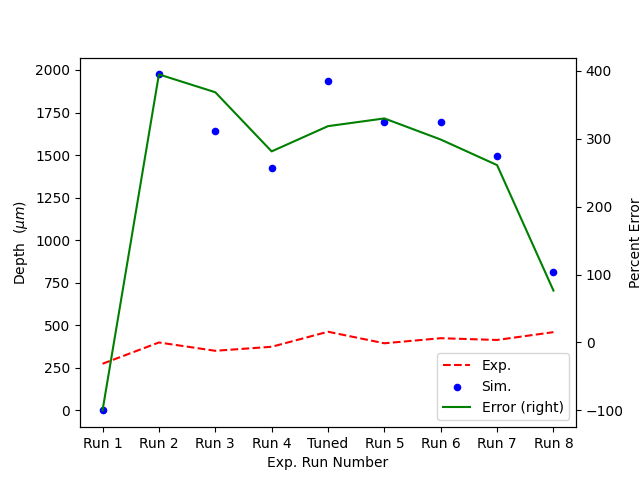
\includegraphics[width=\textwidth]{melt_track_val_baseline_depth}
\caption{\centering}
\label{fig:melt_track_val_baseline_depth}
\end{subfigure}
\begin{subfigure}[c]{0.45\textwidth}\centering
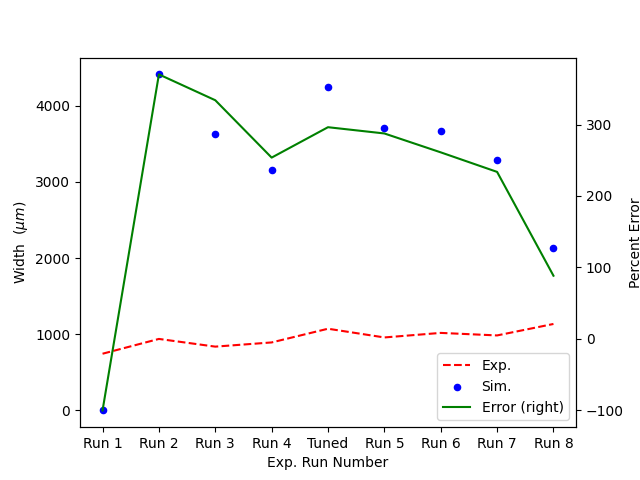
\includegraphics[width=\textwidth]{melt_track_val_baseline_width}
\caption{\centering}
\label{fig:melt_track_val_baseline_width}
\end{subfigure}
\caption{Comparison of experimental and simulated results for validation points with 
generic literature values for the aluminum material dataset. \hl{(\textbf{a}) Melt track 
depth; (\textbf{b}) melt track width.}}
%confirmed
\label{fig:melt_track_val_baseline}
\end{figure}

Where the red dashed line is the experimental results, the blue dots are the simulation 
predictions, and the green line is the error when comparing the simulated results to the 
experimental results.
These results show that over the nine initial parameter sets, when a melt track was 
developed, the average absolute value of the error in the depth was approximately 290\%, 
and the average error in the width was approximately 265\%.  To put this into terms of the 
response variable of the search algorithm, the sum of the width and depth error would be 
555\% combined error.
Additionally, the first run was unable to develop a melt pool, which is contrary to the 
experiments where all the parameter sets had a stable melt track.  These results 
corroborate the results of Figure \ref{fig:response_complete}, which showed that the 
 initial dataset of material properties 
found in the literature is wholly inadequate for simulating the process at hand.  % English 
%Editor: Please verify that the intended meaning has been retained.
% Edited to retain meaning


In contrast to these results, the material dataset found in Table 
\ref{tab:7000_mat_prop_complete} was used to simulate each parameter set, and the 
results can be seen in Figure \ref{fig:melt_track_val}.

\vspace{-12pt}
\begin{figure}[H]
	\begin{subfigure}[c]{0.45\textwidth}
	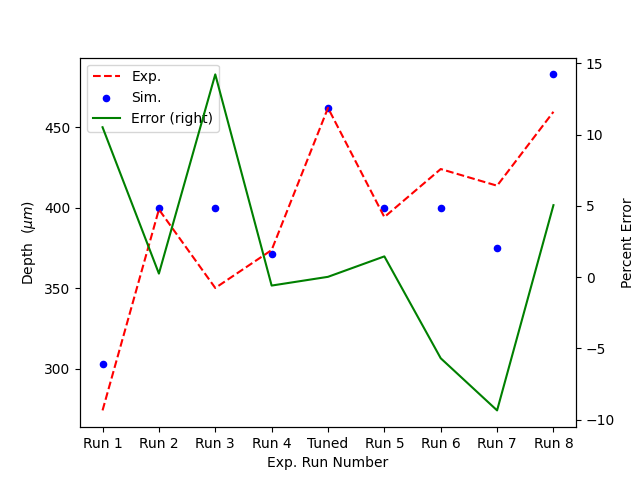
\includegraphics[width=\textwidth]{melt_track_val_depth}
	\caption{\centering}
	\label{fig:melt_track_val_depth}
	\end{subfigure}
		\begin{subfigure}[c]{0.45\textwidth}
		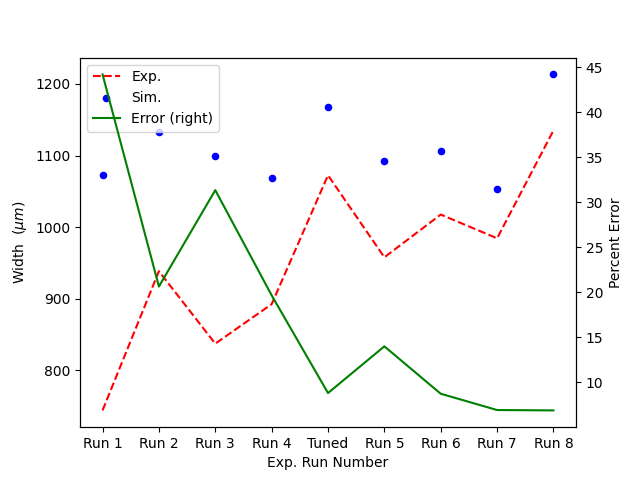
\includegraphics[width=\textwidth]{melt_track_val_width}
		\caption{\centering}
		\label{fig:melt_track_val_width}
		\end{subfigure}
	\caption{Comparison of experimental and simulated results for laser processing 
	parameter validation points with optimized values for the aluminum material dataset. 
	\hl{(\textbf{a}) Melt track depth; (\textbf{b})~melt track width.}}
	%confirmed
	\label{fig:melt_track_val}
\end{figure}
Where the red dashed line is the experimental results, the blue dots are the simulation predictions, and the green line is the error when comparing the simulated results to the experimental results.
These results show the average error in the width was approximately 17\% and the average error in the depth was approximately 5\%, which creates a combined error of only 22\%.  These results show that the optimized dataset is better at predicting the combined error of the simulation by over 500\%.  This results in a simulation that can be leveraged more intensely during the process development and build qualification process.  
These results are from a wide parameter set that encompasses most of the usable 
parameter space for the deposition found experimentally.  This improvement in accuracy 
will 
allow for greater application of the model in the determination of an optimized 
parameter set for a given build.  In addition, the model is seen to be more accurate at 
parameters above the parameter used during the optimization.  This leads to the 
conclusion that if a more accurate simulation is needed, the optimization should be 
conducted at a parameter set near the desired parameter set.
%\FloatBarrier

\section{Discussion}
\label{sec:disucssion}
\label{discussion}

After the simulation developed was shown to properly model the laser \ac{DED} process for a material where the material properties were known, Ti-64, it was understood that the model held to the fundamental physics equations which the model was developed upon and any assumptions in the model were accurate enough to produce accurate results.  This was detailed in Section \ref{model_description}. 
If the material properties did not have a drastic effect on the results of the model, then a 
generic set of aluminum material properties could have been collected and been sufficient 
for the targeted alloy, 7050.  This proved not to be the case, as was expected, due to the 
range of alloying elements in aluminum alloys and their dramatic effect on the material 
properties.  This resulted in effort needing to be exerted to obtain an accurate model for 
the desired 7050 alloy.

The Nelder--Mead algorithm proved to be an efficient method for finding the material 
properties dataset which produced accurate results.  Though more efficient than 
traditional \ac{FEA}, the model still is slow, taking several hours to produce the needed 
results.  This means that the search algorithm selected needed to be efficient and does not 
require numerous queries to achieve a minimum error.  The process of finding the 
derivative of the error function in this search would be possible if several new data points 
were selected around the point of interest resulting in the ability to find the first and 
second derivatives.  This would greatly increase the number of simulation runs required, 
exponentially increasing the time required for the search algorithm to converge.  This 
precluded the common multidimensional algorithms of the conjugate gradient method, 
full Newton method, Davidon--Fletcher--Powell, and 
Broyden--Fletcher--Goldfard--Shanno method.  Additionally, other methods that do not 
require knowledge of the gradient such as Powell's method and line searches typically 
require many more iterations to reach a minimum.  % English Editor: Please verify that the 
%intended meaning has been retained.
%confirmed
Therefore, if the derivatives are not known or the derivatives are not continuous, then the 
Nelder--Mead algorithm should be attempted first	\cite{extremeoptimization}.  Upon 
efficient convergence of the Nelder--Mead algorithm, there was no need to investigate 
other optimization algorithms.

Upon minimization of the error, the results shown in Table \ref{tab:7000_mat_prop_complete} can be compared to \mbox{Table \ref{tab:starting_mat_prop_complete}} to see the difference between the properties that were found for a generic 
alloy and that of the optimized properties.  Two main observations can be made when comparing the results.


The first is that the laser diameter is approximately half that of the starting value.  This 
derives from the difficulty in measuring the diameter of the laser without the appropriate 
dedicated equipment.  In this experiment, the starting laser diameter was selected based 
on experimentation where the laser was scanned on the surface of the substrate.  The 
width of the melt track was measured and used as the laser diameter, confounding the 
laser width with the processing parameter and the material properties.  This rudimentary 
method was a way to cheaply and quickly obtain an approximation of the laser diameter 
but was expected to improperly estimate the laser diameter.  This is due to the dependence 
of the absorbance of the laser on the material, namely its thermal conductivity and specific 
heat as well as the processing parameters.  Specialized equipment could have eliminated 
this variable; however, this is expensive, and it did not significantly affect the convergence 
rate of the Nelder--Mead algorithm.  

Secondly, it is critical to review the difference between the alloys where the generic 
material properties were taken from and the experimentally used material.  The generic 
material properties dataset came from combining the data from pure 
aluminum~\cite{leitner_thermophysical_2017, boyden_temperature_2006}.  When adding 
alloying elements, this can have a drastic effect on the material properties.  In this 
experiment, the alloy of 7050 was used, which contains alloying elements of  copper 
(2.3\%), magnesium (2.3\%), zinc (6.2\%), and zirconium (0.12\%).  This addition of 
alloying elements affected the material properties in the following ways.  Firstly, the laser 
absorption at the liquidus temperature for the optimized dataset was triple that of the 
generic dataset.  Secondly, the specific heat at 733~$^{\circ}$C of the optimized dataset 
was also nearly triple that of the generic dataset. % English Editor: Please verify that the 
%intended meaning has been retained.
%confirmed
Conversely, at 
922~$^{\circ}$C, the generic dataset was triple that of the optimized dataset values.  Lastly, 
the thermal conductivity of the optimized dataset was about double that of the generic 
dataset at 1491~$^{\circ}$C.  These differences most likely arise from the alloying elements 
changing the lattice structure of the aluminum altering its material properties.

The model in this work was developed in response to a need from those developing processing parameters and path plans for the metal \ac{AM} process.  They needed a model that was capable of quickly simulating the heat flow and buildup for a range of path plans and processing parameters.
This will allow researchers to more efficiently test a wider range of parameters and path plans to better find a global optimal value as opposed to the local optimization which might be obtained with a smaller scale set of parameters or path plans, both experimental and simulated.
With the current target of an efficient predictor of the thermal history completed and an 
optimized input dataset for the high-strength aluminum, it is possible to expand this 
model to predict more components of the build and increase its~usefulness.

The next target for the model is to add a prediction of the microstructure of the material.  This is particularly important for the aluminum alloy investigated in this paper because it is the main driving factor as to the expected performance of the final part~\cite{guoMicrostructureMechanicalProperties2022}.
To predict the microstructural makeup of an \ac{AM} build, it is necessary to first find the thermal history due to the tight linking between the thermal history, cooling rates, and microstructure that is developed.  After this, a range of models, both deterministic and probabilistic, can be used to predict the final microstructural makeup of a completed \ac{AM} build~\cite{tanMicrostructureModellingMetallic2020}.  These results can then be used to predict the final part performance.  Moving forward, various methods of predicting the microstructure of the completed build will be evaluated as an intermediate step to estimating the ultimate performance of the component.



\section{Conclusions}
\label{sec:conclusions}
\label{conclusions}

This work shows that the Nelder--Mead search algorithm is an appropriate 
multidimensional search algorithm for the determination of an optimal dataset for 
improved simulation accuracy.  
It was capable of reducing the error of the simulated melt track depth and width of a set of processing parameters as measured by the sum of the error in the width and depth measurements (Equation \eqref{eqn:response}) from over 600\% for a generic aluminum alloy to 9.1\%.
This was verified using a range of laser processing parameters to verify the effectiveness 
over a processing window.  This verified the results, using the same error measurement, 
and the average error was improved by over 500\%
as shown in \mbox{Figures \ref{fig:melt_track_val_baseline} and 
\ref{fig:melt_track_val}}, which used datasets from literature (Table 
\ref{tab:starting_mat_prop_complete}) and the optimized dataset (Table 
\ref{tab:7000_mat_prop_complete}), respectively.  
It was found that the values of the laser absorption at the liquidus temperature and the 
specific heat at 733~$^{\circ}$C for the optimized dataset were triple that of the generic 
dataset.  Conversely, at 922~$^{\circ}$C, the generic dataset was triple that of the 
optimized dataset values.  The thermal conductivity of the optimized dataset was about 
double that of the generic dataset at 1491~$^{\circ}$C.  Lastly, the crudely estimated laser 
diameter  % English Editor: Please verify that the intended meaning has been retained. 
%confirmed
was nearly double that of the optimized input dataset.
This methodology can be used to develop accurate simulations for any material that is not well published or to increase the accuracy of a simulation that utilizes approximations of first principles to increase its efficiency.



\vspace{6pt} 

%%%%%%%%%%%%%%%%%%%%%%%%%%%%%%%%%%%%%%%%%%
% Aaron Flood, Rachel Boillat, Sriram Isanaka and Frank Liou
\authorcontributions{Conceptualization, A.F. and F.L.; methodology, A.F. and F.L.; 
software, A.F.; validation, A.F. and R.B.; formal analysis, A.F.; investigation, A.F., R.B., and 
S.I.; resources, F.L.; data curation, A.F. and R.B.; writing---original draft preparation, A.F. 
and F.L.; writing---review and editing, A.F. and F.L.; visualization, A.F.; supervision, S.I. 
and F.L.; project administration, F.L.; funding acquisition, F.L. All authors have read and 
agreed to the published version of the manuscript.
All authors have read and agreed to the published version of the manuscript.
}

\funding{This research was partially funded by the National Science Foundation Grants CMMI 1625736 and EEC 1937128, Intelligent Systems Center and Material Research Center at Missouri S\&T. Their financial support is greatly appreciated.}

\dataavailability{All data generated or analyzed during this study are included in this published article.} 

\conflictsofinterest{The authors declare no conflicts of interest.} 


\begin{adjustwidth}{-\extralength}{0cm}	
\reftitle{References}

%\bibliography{references}

\begin{thebibliography}{999}

\bibitem[Neittaanm{\"a}ki and
  Rantalainen(2023)]{neittaanmakiImpactScientificComputing2023}
Neittaanm{\"a}ki, P.; Rantalainen, M.L. (Eds.).
{\em Impact of Scientific Computing on Science and Society}; Computational Methods in Applied Sciences; Springer International Publishing: Cham, \hl{Switzerland,} %MDPI: newly information added; please confirm; highlight below same as this
%confirmed
2023; Volume~58.
{\url{https://doi.org/10.1007/978-3-031-29082-4}}.

\bibitem[Qian and Wang(2020)]{qianSubrapidSolidificationStudy2020}
Qian, H.; Wang, W.
Sub-Rapid Solidification Study of Silicon Steel by Using Dip Test Technique. 
In \emph{TMS 2020 149th Annual Meeting \& Exhibition Supplemental Proceedings}; The Minerals, Metals \& Materials Society, Ed.; Springer International Publishing: Cham, \hl{Switzerland,} 2020; \mbox{pp. 39--46}.
{\url{https://doi.org/10.1007/978-3-030-36296-6_4}}.
% confirmed

\bibitem[Wei et~al.(2020)Wei, Mukherjee, Zhang, Zuback, Knapp, De, and DebRoy]{weiMechanisticModelsAdditive2020}
Wei, H.; Mukherjee, T.; Zhang, W.; Zuback, J.; Knapp, G.; De, A.; DebRoy, T.
Mechanistic Models for Additive Manufacturing of Metallic Components.
{\em Prog. Mater. Sci.} {\bf 2020}, \emph{\hl{116}}, 100703.
{\url{https://doi.org/10.1016/j.pmatsci.2020.100703}}.
% confirmed

\bibitem[Ansari and Salamci(2021)]{ansariSelectiveLaserMelting2022}
Ansari, P.; Salamci, M.U.
On the Selective Laser Melting Based Additive Manufacturing of  AlSi\textsubscript{10}Mg: The Process Parameter Investigation through Multiphysics Simulation and Experimental Validation.
{\em J. Alloy. Compd.} {\bf 2021}, {\em 890},~161873.
{\url{https://doi.org/10.1016/j.jallcom.2021.161873}}.

\bibitem[Ning et~al.(2020)Ning, Praniewicz, Wang, Dobbs, and Liang]{ningAnalyticalModelingPart2020}
Ning, J.; Praniewicz, M.; Wang, W.; Dobbs, J.R.; Liang, S.Y.
Analytical Modeling of Part Distortion in Metal Additive Manufacturing.
{\em  Int. J. Adv. Manuf. Technol.}
{\bf 2020}, {\em 107},~49--57.
{\url{https://doi.org/10.1007/s00170-020-05065-8}}.

\bibitem[Promoppatum and Uthaisangsuk(2021)]{promoppatumPartScaleEstimation2021}
Promoppatum, P.; Uthaisangsuk, V.
Part Scale Estimation of Residual Stress Development in Laser Powder Bed Fusion Additive Manufacturing of Inconel 718. {\em Finite Elem. Anal. Des.} {\bf 2021}, {\em 189},~103528.
{\url{https://doi.org/10.1016/j.finel.2021.103528}}.

\bibitem[Ning et~al.(2020)Ning, Sievers, Garmestani, and Liang]{ningAnalyticalModelingPart2020a}
Ning, J.; Sievers, D.E.; Garmestani, H.; Liang, S.Y.
Analytical Modeling of Part Porosity in Metal Additive Manufacturing.
{\em Int. J. Mech. Sci.} {\bf 2020}, {\em 172},~105428.
{\url{https://doi.org/10.1016/j.ijmecsci.2020.105428}}.

\bibitem[Wang et~al.(2020)Wang, Ning, and Liang]{wangPredictionLackoffusionPorosity2021}
Wang, W.; Ning, J.; Liang, S.Y.
Prediction of Lack-of-Fusion Porosity in Laser Powder-Bed Fusion Considering Boundary Conditions and Sensitivity to Laser Power Absorption.
{\em  Int. J. Adv. Manuf. Technol.}
{\bf 2020}, {\em 112},~61--70.
{\url{https://doi.org/10.1007/s00170-020-06224-7}}.

\bibitem[Lin et~al.(2020)Lin, Shen, Wu, Hwang, and Lee]{linProcessOptimizationDirected2020}
Lin, P.Y.; Shen, F.C.; Wu, K.T.; Hwang, S.J.; Lee, H.H.
Process Optimization for Directed Energy Deposition of {{SS316L}} Components.
{\em  Int. J. Adv. Manuf. Technol.}
{\bf 2020}, {\em 111},~1387--1400.
{\url{https://doi.org/10.1007/s00170-020-06113-z}}.

\bibitem[Wang and Chen(2020)]{wangClosedLoopHighFidelitySimulation2021}
Wang, D.; Chen, X.
Closed-{{Loop High-Fidelity Simulation Integrating Finite Element Modeling with Feedback Controls}} in {{Additive Manufacturing}}.
{\em J. Dyn. Syst. Meas. Control} {\bf 2020}, {\em 143},~021006.
{\url{https://doi.org/10.1115/1.4048364}}.

\bibitem[Roy and Wodo(2020)]{royDatadrivenModelingThermal2020}
Roy, M.; Wodo, O.
Data-Driven Modeling of Thermal History in Additive Manufacturing.
{\em Addit. Manuf.} {\bf 2020}, {\em 32},~101017.
{\url{https://doi.org/10.1016/j.addma.2019.101017}}.

\bibitem[Moges et~al.(2020)Moges, Yang, Jones, Feng, Witherell, and Lu]{mogesHYBRIDMODELINGAPPROACH2020}
Moges, T.; Yang, Z.; Jones, K.; Feng, S.; Witherell, P.; Lu, Y.
Hybrid Modeling Approach for Melt Pool Prediction in Laser Powder Bed Fusion Additive Manufacturing.
\emph{\hl{J. Comput. Inf. Sci. Eng.}}
{\bf \hl{2021}}\hl{, \emph{21}, 050902.}
% confirmed

\bibitem[Daryabeigi(2011)]{daryabeigiThermalPropertiesAccurate2011}
Daryabeigi, K.
Thermal {{Properties}} for {{Accurate Thermal Modeling}},  \colorbox{green}{2011.} %MDPI: Please provide more information about the type of the article, such as book (please provide the name of the publisher and location of it), online resource (please provide the URL of the website and the date it was accessed (day, month, year)), or journal article (please provide the name of the journal, the year and volume it published, and the page number).
{\url{https://tfaws.nasa.gov/TFAWS11/Proceedings/Thermal%20Properties%20Testing%20Course.pdf}}.
({accessed on: 31 March 2020}).
%If no, please provide the URL of the website and the date it was accessed (Date Month Year) at least 
% This is a powerpoint slide deck for a presentation which can be found at the above url

\bibitem[Zhu et~al.(2020)Zhu, Liu, and Yan]{zhuMachineLearningMetal2020}
Zhu, Q.; Liu, Z.; Yan, J.
Machine Learning for Metal Additive Manufacturing: {{Predicting}} Temperature and Melt Pool Fluid Dynamics Using Physics-Informed Neural \hl{Networks.}
%MDPI: please confirm we removed extra coontent
% confirmed
{\em arXiv} {\bf 2020}, arXiv:2008.13547.


\bibitem[Zobeiry and Humfeld(2021)]{zobeiryPhysicsinformedMachineLearning2021}
Zobeiry, N.; Humfeld, K.D.
A Physics-Informed Machine Learning Approach for Solving Heat
  Transfer Equation in Advanced Manufacturing and Engineering Applications.
{\em Eng. Appl. Artif. Intell.} {\bf 2021},
  {\em 101},~104232.
\newblock {\url{https://doi.org/10.1016/j.engappai.2021.104232}}.

\bibitem[Meng et~al.(2020)Meng, McWilliams, Jarosinski, Park, Jung, Lee, and
  Zhang]{mengMachineLearningAdditive2020}
Meng, L.; McWilliams, B.; Jarosinski, W.; Park, H.Y.; Jung, Y.G.; Lee, J.;
  Zhang, J.
\newblock Machine {{Learning}} in {{Additive Manufacturing}}: {{A Review}}.
\newblock {\em JOM} {\bf 2020}, {\em 72},~2363--2377.
\newblock {\url{https://doi.org/10.1007/s11837-020-04155-y}}.

\bibitem[Wang et~al.(2020)Wang, Tan, Tor, and
  Lim]{wangMachineLearningAdditive2020}
Wang, C.; Tan, X.; Tor, S.; Lim, C.
\newblock Machine Learning in Additive Manufacturing: {{State-of-the-art}} and
  Perspectives.
\newblock {\em Addit. Manuf.} {\bf 2020}, {\em 36},~101538.
\newblock {\url{https://doi.org/10.1016/j.addma.2020.101538}}.

\bibitem[Welsch et~al.(1993)Welsch, Boyer, and Collings]{welschgerhard_1993}
Welsch, G.; Boyer, R.; Collings, E.
{\em Materials Properties Handbook: Titanium Alloys};
\hl{ASM International: Materials Park, OH} %MDPI: please add location of publisher
% updated
1993.

\bibitem[Boivineau et~al.(2006)Boivineau, Cagran, Doytier, Eyraud, Nadal,
  Wilthan, and Pottlacher]{boivineau_2006}
Boivineau, M.; Cagran, C.; Doytier, D.; Eyraud, V.; Nadal, M.H.; Wilthan, B.; Pottlacher, G.
\newblock Thermophysical {{Properties}} of {{Solid}} and {{Liquid Ti-6Al-4V}}
({{TA6V}}) {{Alloy}}.
\newblock {\em Int. J. Thermophys.} {\bf 2006}, {\em
  27},~507--529.
\newblock {\url{https://doi.org/10.1007/PL00021868}}.

\bibitem[Fan and Liou(2012)]{fan_2012}
Fan, Z.; Liou, F.
Numerical Modeling of the Additive Manufacturing (AM) Processes of Titanium Alloy. 
In {\em Titanium Alloys---Towards Achieving Enhanced Properties for Diversified Applications}; 
Amin,  A.N., Ed.; InTech: \hl{London, UK,} 2012.
{\url{https://doi.org/10.5772/34848}}.
% confirmed

\bibitem[Lundberg(1994)]{lundberg_material_1994}
Lundberg, S.
Material Aspects of Fire Design, \colorbox{green}{1994.} %MDPI: Please provide more information about the type of the article, such as book (please provide the name of the publisher and location of it), online resource (please provide the URL of the website and the date it was accessed (day, month, year)), or journal article (please provide the name of the journal, the year and volume it published, and the page number).
{\url{https://aluminium-guide.com/en/en/talat-lectures/}}.
({accessed on: 23 March 2020}).
%If no, please provide the URL of the website and the date it was accessed (Date Month Year) at least 
% This is an online resource

\bibitem[Leitner et~al.(2017)Leitner, Leitner, Schmon, Aziz, and
  Pottlacher]{leitner_thermophysical_2017}
Leitner, M.; Leitner, T.; Schmon, A.; Aziz, K.; Pottlacher, G.
\newblock Thermophysical {{Properties}} of {{Liquid Aluminum}}.
\newblock {\em Metall. Mater. Trans. A} {\bf 2017}, {\em
  48},~3036--3045.
\newblock {\url{https://doi.org/10.1007/s11661-017-4053-6}}.

\bibitem[jma()]{jmatpro}
JMatPro.
Available online: \url{https://www.sentesoftware.co.uk/jmatpro} (\hl{accessed on: 14 September 2022}%MDPI: Please add the access date (Format: Date Month Year). e.g., (accessed on 1 January 2020).
% updated
).

\bibitem[Liu et~al.(2020)Liu, Long, Zhang, Zhao, Zhao, Feng, Chen, and
  Ma]{liuStudyPredictionTensile2020}
\textls[-15]{Liu, S.; Long, M.; Zhang, S.; Zhao, Y.; Zhao, J.; Feng, Y.; Chen, D.; Ma, M.
\newblock Study on the Prediction of Tensile Strength and Phase Transition for
  Ultra-High Strength Hot Stamping Steel.
\newblock {\em J. Mater. Res. Technol.} {\bf 2020}, {\em
  9},~14244--14253.
\newblock {\url{https://doi.org/10.1016/j.jmrt.2020.10.043}}.}

\bibitem[Chen et~al.(2023)Chen, Yu, Hou, Zhu, and
  Zhang]{chenMicrostructurePropertiesIronbased2023}
Chen, Z.; Yu, Y.; Hou, J.; Zhu, P.; Zhang, J.
\newblock Microstructure and Properties of Iron-Based Surfacing Layer Based on
  {{JmatPro}} Software Simulation Calculation.
\newblock {\em Vibroeng. Procedia} {\bf 2023}, {\em 50},~180--186.
\newblock {\url{https://doi.org/10.21595/vp.2023.23400}}.

\bibitem[Geng et~al.(2022)Geng, Cheng, Wang, Peng, Ullah, Wang, and
  Wu]{gengDatadrivenMachineLearning2022}
Geng, X.; Cheng, Z.; Wang, S.; Peng, C.; Ullah, A.; Wang, H.; Wu, G.
\newblock A Data-Driven Machine Learning Approach to Predict the Hardenability
  Curve of Boron Steels and Assist Alloy Design.
\newblock {\em J. Mater. Sci.} {\bf 2022}, {\em
  57},~10755--10768.
\newblock {\url{https://doi.org/10.1007/s10853-022-07132-9}}.

\bibitem[Qi(2020)]{qiHighStrengthLi2020}
Qi, Y.
\newblock A High Strength {{Al}}\textendash{{Li}} Alloy Produced by Laser
  Powder Bed Fusion\_ {{Densification}}, Microstructure, and Mechanical
  Properties.
\newblock {\em Addit. Manuf.} {\bf 2020}, {\em 35},~101346.
\newblock {\url{https://doi.org/doi.org/10.1016/j.addma.2020.101346}}.

\bibitem[Weiss(2019{\natexlab{a}})]{weissImprovedHighTemperatureAluminum2019}
Weiss, D.
\newblock Improved {{High-Temperature Aluminum Alloys Containing Cerium}}.
\newblock {\em J. Mater. Eng. Perform.} {\bf 2019},
  {\em 28},~1903--1908.
\newblock {\url{https://doi.org/10.1007/s11665-019-3884-2}}.

\bibitem[Weiss(2019{\natexlab{b}})]{weissDevelopmentsAluminumScandiumCeramicAluminumScandiumCerium2019}
Weiss, D.
Developments in Aluminum-Scandium-Ceramic and Aluminum-Scandium-Cerium Alloys. 
In {\em Light Metals 2019}; Chesonis, C., Ed.; 
Springer International Publishing: Cham, \hl{Switzerland,} 2019; \mbox{pp. 1439--1443}.
{\url{https://doi.org/10.1007/978-3-030-05864-7\_180}}.
% confirmed

\bibitem[Singh(2017)]{singhAdditiveManufacturing4047}
Singh, A. Additive Manufacturing of Al 4047 and Al 7050 Alloys Using Direct Laser Metal Deposition Process.
Ph.D. Thesis, Wayne State University, Detroit, MI, \hl{USA}, 2017.
% confirmed

\bibitem[Han(2012)]{Han2012}
Han, J.C.
{\em Analytical Heat Transfer}; CRC Press:  \hl{Boca Raton, FL, USA,} %We added the location of publisher. Please confirm
% confirmed
2012.

\bibitem[Mills(2002)]{mills_2002}
Mills, K.
Recommended Values of Thermophysical Properties for Selected Commercial Alloys. 
In {\em Recommended Values of Thermophysical Properties for Selected Commercial Alloys}; 
Woodhead Publishing Series in Metals and Surface Engineering; 
\hl{Woodhead Publishing: Cambridge UK} 2002; pp. 211--217.
% updated

\bibitem[Kurzynowski et~al.(2019)Kurzynowski, Stopyra, Gruber,
  Zi{\'o}{\l}kowski, Ku{\'z}nicka, and
  Chlebus]{kurzynowskiEffectScanningSupport2019}
Kurzynowski, T.; Stopyra, W.; Gruber, K.; Zi{\'o}{\l}kowski, G.; Ku{\'z}nicka,
  B.; Chlebus, E.
\newblock Effect of {{Scanning}} and {{Support Strategies}} on {{Relative
  Density}} of {{SLM-ed H13 Steel}} in {{Relation}} to {{Specimen Size}}.
\newblock {\em Materials} {\bf 2019}, {\em 12},~239.
\newblock {\url{https://doi.org/10.3390/ma12020239}}.

\bibitem[Nelder and Mead(1965)]{nelder_1965}
Nelder, J.A.; Mead, R.
\newblock A {{Simplex Method}} for {{Function Minimization}}.
\newblock {\em  Comput. J.} {\bf 1965}, {\em 7},~308--313.
\newblock {\url{https://doi.org/10.1093/comjnl/7.4.308}}.

\bibitem[Wang and Shoup(2011)]{wang_2011}
Wang, P.C.; Shoup, T.E.
\newblock Parameter Sensitivity Study of the {{Nelder}}\textendash{{Mead
  Simplex Method}}.
\newblock {\em Adv. Eng. Softw.} {\bf 2011}, {\em
  42},~529--533.
\newblock {\url{https://doi.org/10.1016/j.advengsoft.2011.04.004}}.

\bibitem[{Joseph R. Davis}(2001)]{joseph_r_davis_aluminum_2001}
Davis, J.R.
Aluminum and Aluminum Alloys Davis. 
In {\em Alloying: Understanding the Basics}; \hl{ASM International}: 2001; pp. 351--416.
% confirmed

\bibitem[Ulbirch(2014)]{ulbrich_wire_2014}
Ulbirch. 6000 \& 7000 {{Series Aluminum Alloy}}, \colorbox{green}{2014.} %MDPI: Please provide more information about the type of the article, such as book (please provide the name of the publisher and location of it), online resource (please provide the URL of the website and the date it was accessed (day, month, year)), or journal article (please provide the name of the journal, the year and volume it published, and the page number).
{\url{https://www.ulbrich.com/alloys/6000-7000-series-aluminum-alloys/}}.
{accessed on: 11 June 2020}
%If no, please provide the URL of the website and the date it was accessed (Date Month Year) at least 
% updated

\bibitem[ASM(2022)]{matweb}
ASM.
Aluminum 6061-{{T6}}; 6061-{{T651}}. 2022
Available online: \url{http://asm.matweb.com/search/SpecificMaterial.asp?bassnum=MA6061T6} (\hl{accessed on}).

\bibitem[AmesWeb(2022)]{amesweb}
AmesWeb.
Aluminum 6061 Material Properties. 2022
Available online: \url{https://amesweb.info/Materials/Aluminum-6061-Properties.aspx} (\hl{accessed on: 5 November 2020}).
% updated

\bibitem[Schmitz et~al.(2012)Schmitz, Hallstedt, Brillo, Egry, and Schick]{schmitz_density_2012}
Schmitz, J.; Hallstedt, B.; Brillo, J.; Egry, I.; Schick, M.
Density and Thermal Expansion of Liquid {{Al}}\textendash{{Si}} Alloys.
\newblock {\em J. Mater. Sci.} {\bf 2012}, {\em 47},~3706--3712.
\newblock {\url{https://doi.org/10.1007/s10853-011-6219-8}}.

\bibitem[Funck et~al.(2014)Funck, Nett, and Ostendorf]{funck_tailored_2014}
Funck, K.; Nett, R.; Ostendorf, A.
\newblock Tailored {{Beam Shaping}} for {{Laser Spot Joining}} of {{Highly
  Conductive Thin Foils}}.
\newblock {\em Phys. Procedia} {\bf 2014}, {\em 56},~750--758.
\newblock {\url{https://doi.org/10.1016/j.phpro.2014.08.082}}.

\bibitem[Boyden and Zhang(2006)]{boyden_temperature_2006}
Boyden, S.B.; Zhang, Y.
\newblock Temperature and {{Wavelength-Dependent Spectral Absorptivities}} of
  {{Metallic Materials}} in the {{Infrared}}.
\newblock {\em J. Thermophys. Heat Transf.} {\bf 2006}, {\em
  20},~9--15.
\newblock {\url{https://doi.org/10.2514/1.15518}}.

\bibitem[{El-Hameed} et~al.(2017){El-Hameed}, {Abdel-Aziz}, and
  {El-Tokhy}]{el-hameed_anodic_2017}
{El-Hameed}, A.M.A.; {Abdel-Aziz}, Y.A.; {El-Tokhy}, F.S.
\newblock Anodic {{Coating Characteristics}} of {{Different Aluminum Alloys}}
  for {{Spacecraft Materials Applications}}.
\newblock {\em Mater. Sci. Appl.} {\bf 2017}, {\em 8},~197--208.
\newblock {\url{https://doi.org/10.4236/msa.2017.82013}}.

\bibitem[Flood and Liou(2023)]{floodSensitivityAnalysisDirected2023}
Flood, A.; Liou, F.
\newblock Sensitivity {{Analysis}} of {{Directed Energy Deposition Simulation
  Results}} to {{Aluminum Material Properties}}.
\newblock {\em 3D Print. Addit. Manuf.} 2023, {\em  accepted}.

\bibitem[Optimization()]{extremeoptimization}
Optimization, E. Available online: \url{https://www.extremeoptimization.com/documentation/mathematics/optimization/multidimensional-optimization} (\hl{accessed on 16 October 2023}).
% updated

\bibitem[Guo et~al.(2022)Guo, Li, Pan, and
  Zhou]{guoMicrostructureMechanicalProperties2022}
Guo, X.; Li, H.; Pan, Z.; Zhou, S.
\newblock Microstructure and Mechanical Properties of Ultra-High Strength
  {{Al-Zn-Mg-Cu-Sc}} Aluminum Alloy Fabricated by Wire + Arc Additive
  Manufacturing.
\newblock {\em J. Manuf. Process.} {\bf 2022}, {\em
  79},~576--586.
\newblock {\url{https://doi.org/10.1016/j.jmapro.2022.05.009}}.

\bibitem[Tan et~al.(2019)Tan, Sing, and
  Yeong]{tanMicrostructureModellingMetallic2020}
Tan, J.H.K.; Sing, S.L.; Yeong, W.Y.
Microstructure Modelling for Metallic Additive Manufacturing: A Review.
{\em Virtual Phys. Prototyp.} {\bf 2019}, {\em 15},~87--105.
{\url{https://doi.org/10.1080/17452759.2019.1677345}}.

\end{thebibliography}


\PublishersNote{}
\end{adjustwidth}

\end{document}
